% Modeled after sample-sigplan.tex
\documentclass[sigplan,anonymous,review,10pt]{acmart}
%\documentclass[sigplan,10pt]{acmart}
%% \BibTeX command to typeset BibTeX logo in the docs
\AtBeginDocument{%
  \providecommand\BibTeX{{%
    Bib\TeX}}}
\setcopyright{acmlicensed}
\copyrightyear{2018}
\acmYear{2018}
\acmDOI{XXXXXXX.XXXXXXX}
%% These commands are for a PROCEEDINGS abstract or paper.
\acmConference[Onward!]{Onward!}{Oct.\ 20-25, 2024}{Pasadena, CA}
\acmISBN{978-1-4503-XXXX-X/18/06}
% ============================================================
% ============================================================
\usepackage{xspace}
\usepackage{graphicx}
\graphicspath{{figures/}}
% ============================================================
%% Uncomment the next few lines to get sf url links:
%\usepackage{url}            
%\makeatletter
%\def\url@leostyle{%
%  \@ifundefined{selectfont}{\def\UrlFont{\sf}}{\def\UrlFont{\small\sffamily}}}
%\makeatother
%\urlstyle{leo} % Now actually use the newly defined style.
%% Choose coloured or b/w links:
%\usepackage[pdftex,colorlinks=true,pdfstartview=FitV,
% linkcolor=black,citecolor=black,urlcolor=black]{hyperref}
%\usepackage{hyperref}
\usepackage{needspace}
\newcommand{\needlines}[1]{\Needspace{#1\baselineskip}}
\usepackage{paralist}
% ============================================================
%:Markup macros for proof-reading
\usepackage{ifthen}
\usepackage[normalem]{ulem} % for \sout
\usepackage{xcolor}
\newcommand{\ra}{$\rightarrow$}
\newboolean{showedits}
\setboolean{showedits}{true} % toggle to show or hide edits
%\setboolean{showedits}{false} % toggle to show or hide edits
\ifthenelse{\boolean{showedits}}
{
	\newcommand{\meh}[1]{\textcolor{red}{\uwave{#1}}} % please rephrase
	\newcommand{\ins}[1]{\textcolor{blue}{\uline{#1}}} % please insert
	\newcommand{\del}[1]{\textcolor{red}{\sout{#1}}} % please delete
	\newcommand{\chg}[2]{\textcolor{red}{\sout{#1}}{\ra}\textcolor{blue}{\uline{#2}}} % please change
	\newcommand{\nbe}[3]{
		{\colorbox{#3}{\bfseries\sffamily\scriptsize\textcolor{white}{#1}}}
		{\textcolor{#3}{\sf\small$\blacktriangleright$\textit{#2}$\blacktriangleleft$}}}
}{
	\newcommand{\meh}[1]{#1} % please rephrase
	\newcommand{\ins}[1]{#1} % please insert
	\newcommand{\del}[1]{} % please delete
	\newcommand{\chg}[2]{#2}
	\newcommand{\nbe}[3]{}
}
%
\newcommand\rA[1]{\nbe{Reviewer A}{#1}{cyan}}
\newcommand\rB[1]{\nbe{Reviewer B}{#1}{olive}}
\newcommand\rC[1]{\nbe{Reviewer C}{#1}{magenta}}
\newcommand\ANS[1]{\nbe{Response}{#1}{teal}}

\newcommand{\THE}{\ins{the}\xspace} % "the" missing
\newcommand{\A}{\ins{a}\xspace} % "a" missing
\newcommand{\s}{\ins{s}\xspace} % "s" missing
\newcommand{\COMMA}{\ins{,}\xspace} % "," missing
\newcommand{\THAT}{\chg{which}{that}\xspace} % use "that", not "which"

% ============================================================
%:Box comments/edits
\usepackage[most]{tcolorbox}
\ifthenelse{\boolean{showedits}}
{
  \newtcolorbox{inserted}{%
       title=Inserted text:,
       colframe=blue,colback=blue!5!white,
       breakable,
       leftrule=0mm, 
       bottomrule=0mm,
       rightrule=0mm,
       toprule=0mm,
       arc=0mm, outer arc=0mm,
       oversize
  }
  \newtcolorbox{deleted}{%
       title=Deleted text:,
       colframe=red,colback=red!5!white,
       breakable,
       leftrule=0mm, 
       bottomrule=0mm,
       rightrule=0mm,
       toprule=0mm,
       arc=0mm, outer arc=0mm,
       oversize
  }
  \newtcolorbox{refactored}{%
       % title=Heavily modifed/refactored text:,
       title=Rewritten text:,
       colframe=blue,colback=red!5!white,
       breakable,
       leftrule=0mm, 
       bottomrule=0mm,
       rightrule=0mm,
       toprule=0mm,
       arc=0mm, outer arc=0mm,
       oversize
  }
}{
  \newenvironment{inserted}{}{}
  %\newenvironment{deleted}{ \begin{comment} }{ \end{comment} }
  \let\deleted\comment
  \newenvironment{refactored}{}{} 
}
% ============================================================
%:Put edit comments in a really ugly standout display
%\usepackage{ifthen}
%\usepackage{amssymb} % Avoid error: Command `\Bbbk' already defined.
\newboolean{showcomments}
\setboolean{showcomments}{true}
%\setboolean{showcomments}{false}
\newcommand{\id}[1]{$-$Id: scgPaper.tex 32478 2010-04-29 09:11:32Z oscar $-$}
\newcommand{\yellowbox}[1]{\fcolorbox{gray}{yellow}{\bfseries\sffamily\scriptsize#1}}
\newcommand{\triangles}[1]{{\sf\small$\blacktriangleright$\textit{#1}$\blacktriangleleft$}}
\ifthenelse{\boolean{showcomments}}
%{\newcommand{\nb}[2]{{\yellowbox{#1}\triangles{#2}}}
{\newcommand{\nbc}[3]{
 {\colorbox{#3}{\bfseries\sffamily\scriptsize\textcolor{white}{#1}}}
 {\textcolor{#3}{\sf\small$\blacktriangleright$\textit{#2}$\blacktriangleleft$}}}
 \newcommand{\version}{\emph{\scriptsize\id}}}
{\newcommand{\nbc}[3]{}
 \newcommand{\version}{}}
\newcommand{\nb}[2]{\nbc{#1}{#2}{orange}}
\newcommand{\here}{\yellowbox{$\Rightarrow$ CONTINUE HERE $\Leftarrow$}}
\newcommand\rev[2]{\nb{TODO (rev #1)}{#2}} % reviewer comments
\newcommand\fix[1]{\nb{FIX}{#1}}
\newcommand\todo[1]{\nb{TO DO}{#1}}
%\newcommand\XXX[1]{\nbc{XXX}{#1}{brown}}
%\newcommand\XXX[1]{\nbc{XXX}{#1}{cyan}}
%\newcommand\XXX[1]{\nbc{XXX}{#1}{darkgray}}
%\newcommand\XXX[1]{\nbc{XXX}{#1}{gray}}
%\newcommand\XXX[1]{\nbc{XXX}{#1}{magenta}}
%\newcommand\XXX[1]{\nbc{XXX}{#1}{olive}}
%\newcommand\XXX[1]{\nbc{XXX}{#1}{orange}}
%\newcommand\XXX[1]{\nbc{XXX}{#1}{purple}}
%\newcommand\XXX[1]{\nbc{XXX}{#1}{red}}
%\newcommand\XXX[1]{\nbc{XXX}{#1}{teal}}
%\newcommand\XXX[1]{\nbc{XXX}{#1}{violet}}
% ============================================================
\newboolean{isblinded}
\setboolean{isblinded}{true}
%\setboolean{isblinded}{false}
\ifthenelse{\boolean{isblinded}}
{\newcommand\blind[1]{BLINDED\xspace}}
{\newcommand\blind[1]{#1\xspace}}
% ============================================================
\newcommand{\seclabel}[1]{\label{sec:#1}}
%\newcommand{\secref}[1]{Section~\ref{sec:#1}} <- use \autoref instead!
\newcommand{\figlabel}[1]{\label{fig:#1}}
%\newcommand{\figref}[1]{Figure~\ref{fig:#1}}
\newcommand{\tablabel}[1]{\label{tab:#1}}
%\newcommand{\tabref}[1]{Table~\ref{tab:#1}}
% ============================================================
\newcommand{\ie}{\emph{i.e.},\xspace}
\newcommand{\eg}{\emph{e.g.},\xspace}
\newcommand{\etal}{\emph{et al.}\xspace}
\newcommand{\etc}{\emph{etc.}\xspace}
% ============================================================

% $Author: oscar $
% $Date: 2009-11-06 14:37:12 +0100 (Fri, 06 Nov 2009) $
% $Revision: 29604 $
%=============================================================
% ST80 listings macros
% Adapted from Squeak by Example book
%=============================================================
% If you want >>> appearing as right guillemet, you need these two lines:
%\usepackage[T1]{fontenc}
%\newcommand{\sep}{\mbox{>>}}
% Otherwise use this:
\newcommand{\sep}{\mbox{$\gg$}}
%=============================================================
%:\needlines{N} before code block to force page feed
%\usepackage{needspace}
%\newcommand{\needlines}[1]{\Needspace{#1\baselineskip}}
%=============================================================
%:Listings package configuration for ST80
\usepackage[english]{babel}
%\usepackage{amssymb,textcomp}
\usepackage{listings}
% \usepackage[usenames,dvipsnames]{color}
% \usepackage[usenames]{color}
% \definecolor{source}{gray}{0.95}
\lstdefinelanguage{Smalltalk}{
  % morekeywords={self,super,true,false,nil,thisContext, eachModel}, % This is overkill
  morestring=[d]',
  morecomment=[s]{"}{"},
  alsoletter={\#:},
  escapechar={!},
  literate=
    {BANG}{!}1
    {UNDERSCORE}{\_}1
    % {\\st}{Smalltalk}9 % convenience -- in case \st occurs in code
    % {'}{{\textquotesingle}}1 % replaced by upquote=true in \lstset
    {_}{{$\leftarrow$}}1
    {>>>}{{\sep}}1
    {^}{{$\uparrow$}}1
    {~}{{$\sim$}}1
    {-}{{\sf -\hspace{-0.13em}-}}1  % the goal is to make - the same width as +
    {+}{\raisebox{0.08ex}{+}}1		% and to raise + off the baseline to match -
    {-->}{{\quad$\longrightarrow$\quad}}3
	, % Don't forget the comma at the end!
  tabsize=4
}[keywords,comments,strings]

\definecolor{source}{gray}{0.95}

\lstset{language=Smalltalk,
	basicstyle=\sffamily,
	keywordstyle=\color{black}\bfseries,
%	numbers=left,                   % where to put the line-numbers
%	numberstyle=\footnotesize,      % the size of the fonts that are used for the line-numbers
%	stepnumber=1,                   % the step between two line-numbers. If it is 1 each line will be numbered
%	numbersep=5pt,                  % how far the line-numbers are from the code
%	stringstyle=\ttfamily, % Ugly! do we really want this? -- on
	mathescape=true,
	showstringspaces=false,
	keepspaces=true,
	breaklines=true,
	breakautoindent=true,
	backgroundcolor=\color{source},
	%lineskip={-1pt}, % Ugly hack
	upquote=true, % straight quote; requires textcomp package
	columns=fullflexible} % no fixed width fonts
% In-line code (literal)
% Normally use this for all in-line code:
\newcommand{\st}{\lstinline[mathescape=false,backgroundcolor=\color{white},basicstyle={\sffamily\upshape}]}
% In-line code (latex enabled)
% Use this only in special situations where \ct does not work
% (within section headings ...):
\newcommand{\lst}[1]{{\textsf{\textup{#1}}}}
% Code environments
\lstnewenvironment{code}{%
	\lstset{%
		% frame=lines,
		frame=single,
		framerule=0pt,
		mathescape=false
	}
}{}

% Useful to add a matching $ after code containing a $
% \def\ignoredollar#1{}
%=============================================================

% ============================================================
% Macros for this paper
%\renewcommand{\nbc}[3]{} % To hide reviewer comments
\newcommand\on[1]{\nbc{ON}{#1}{olive}} % add more author macros here
\newcommand\tg[1]{\nbc{TG}{#1}{blue}}
\newcommand\ac[1]{\nbc{AC}{#1}{teal}}
\newcommand\steve[1]{\nbc{Steven}{#1}{red}} % Costiou
\newcommand\ab[1]{\nbc{Alex}{#1}{violet}} % Bergel
\newcommand\tk[1]{\nbc{Timo}{#1}{green}} % Kehrer
\usepackage{caption}
\captionsetup{aboveskip=5pt,belowskip=-10pt} % Adjust the space around figure captions
%\usepackage{enumitem}
%\setlist[description]{font=\itshape}
\newcommand{\GT}{\lst{GT}\xspace} % In case we want to display it differently ...
\newcommand\lmaf{\lst{Ludo\-Move\-Assert\-ion\-Fail\-ure}\xspace}
% ============================================================
% Optionally anonymize selected names
\newboolean{anonymous}
\setboolean{anonymous}{true}
\newcommand\anonymize[2]{\ifthenelse{\boolean{anonymous}}{#2}{#1}\xspace}
\newcommand\feenk{\anonymize{feenk}{anonymous company}}
\newcommand\deet{{\tt deet}\xspace}
% ============================================================
\begin{document}
\title{Moldable Exceptions}
\author{Andrei Chi\c{s}}
\affiliation{%
  \institution{feenk gmbh}
  \city{Wabern}
  \country{Switzerland}}
\email{andrei.chis@feenk.com}
\author{Tudor G\^irba}
\affiliation{%
  \institution{feenk gmbh}
  \city{Wabern}
  \country{Switzerland}}
\email{tudor.girba@feenk.com}
\author{Oscar Nierstrasz}
\affiliation{%
  \institution{feenk gmbh}
  \city{Wabern}
  \country{Switzerland}}
\email{oscar.nierstrasz@feenk.com}

\renewcommand{\shortauthors}{Chi\c{s} et al.}

\begin{abstract}
Debugging is hard.
Debuggers are mostly the same.
They show you a stack, a way to sample the state of the stack, and, if the debugger is live, a way to step through execution.
The standard debugger mostly offers a low-level interface in terms of generic language constructs to track down and fix bugs.
\steve{In the abstract, you say "the standard debugger". Perhaps it is an English subtility that I do not understand and it means "any standard debugger". The problems you mention concern the vast majority of debuggers, everywhere. Even Smalltalk debuggers are in fact very similar to the java debugger and others.}
A custom debugger, such as those developed for specific application domains, offers alternative interfaces more suitable to the specific execution context of the program being debugged.
Contextual debugging views and actions greatly improve our ability to reason about the current problem.
\ab{The abstract implies that "Contextual debugging views" are "custom debuggers". I agree, but it is difficult to grasp from the text.}
Implementing such custom debuggers, however, is non-trivial, and poses a barrier to improving the debugging experience.
In this paper we introduce \emph{moldable exceptions}, a lightweight mechanism to adapt a debugger's interface based on contextual information provided by a raised exception.
We present, through a series of examples, how moldable exceptions can enhance a live programming environment.
\end{abstract}

\keywords{Exceptions, debuggers, customization.}

%\received{20 February 2007}
%\received[revised]{12 March 2009}
%\received[accepted]{5 June 2009}

\maketitle

% ============================================================
\section{Introduction}\label{sec:intro}

\ab{I would add that a similar (albeit much less expressive) behavior could be achieved in other languages by simply overriding toString() to an exception. It is a common practice to have a detailed textual description of exceptions.\\
This textual description is used by the classical Java debugger, but this is limited to a textual representation. Your approach goes much further by having a specific interface and specific actions. Maybe you could mention this in the related work, or in the introduction.}
% [NamingException.java#L400](https://github.com/openjdk/jdk/blob/896107705615a3b9363b7a0a3e6703b20fedef70/src/java.naming/share/classes/javax/naming/NamingException.java#L400)
% [NamingException.java#L424](https://github.com/openjdk/jdk/blob/896107705615a3b9363b7a0a3e6703b20fedef70/src/java.naming/share/classes/javax/naming/NamingException.java#L424)

In the bad old days, all debuggers were the same.
You had commands to sample the current execution state, and you had commands to step through the running code.
Nowadays we have graphical debuggers that show us the run-time stack, and offer buttons instead of commands to step through the code, but they are still all the same.
The trouble with this is that every debugging problem is different, but debuggers all show us the same thing.
\steve{Following the first remark, l.39  you say all debuggers show us the same things, but they also provide us with the same actions: step, break, etc. and it is very limited as you say later for investigating problem-specific things. It also introduces a gap: when investigating specific, non-conventional debugging problems, we have to transform somehow our debugging questions to a sequence of steps and breakpoints etc. that bring us to the information we seek, but it's difficult as it's like using a hammer to break nuts.}

There have been numerous efforts to develop custom debuggers for various application domains and domain-specific languages.
\ab{Line 40: "There have been numerous efforts to develop custom debuggers for various application domains and domain-specific languages." => Can be reinforced with a ref, such as this one: Object-Centric Debugging -- Jorge Ressia, Alexandre Bergel, Oscar Nierstrasz. Proceedings of the 34th International Conference on Software Engineering (ICSE'12)}\nocite{Ress12a}
These custom debuggers provide dedicated views and actions that are tailored to a specific application context.
Building a custom debugger is, however, a non-trivial task, so this does not happen too often.
An \emph{extensible} debugger (such as \deet~\cite{Hans97a}) is designed so that it can be easily extended with new graphical views and debugging operations, but these extensions still represent a significant development effort.
A \emph{moldable debugger}~\cite{Chis15c} is a special kind of extensible debugger that can activate alternative debugger interfaces depending on the current execution context, however the development of these alternative debuggers is still non-trivial.

%\ac{For the abstract/introduction we could emphasise more that even if it is currently possible to have multiple custom debuggers in GT/Pharo, the extension mechanism plays an important role.
%If the cost is high, the chances that developers will do it decreases.
%Maybe a good discussion here would be the extensions for views/searches/actions.
%There the extensions mechanism is different and we created many extensions.
%But even if the debugger is extensible we have only a few custom debuggers as the effort to create one is high.
%We will still need to have standalone debuggers with a higher cost to create in some cases (for example the SmaCC debugger), but in many cases we will benefit from being able to integrate views/actions in the debugger in an easier way.}

%\ac{In a way Moldable Exceptions augments the current extension mechanism for the debugger.
%In the current extension mechanism at each step in the execution we need to determine the list of available debuggers.
%For that we have multiple debuggers registered in the system, and we ask each debugger if it wants to handle the current context or not.
%With moldable exceptions in case we have also an exception in the current context we ask that exception to provide us with a list of of debugging views and actions to add to the current debugger and a list of new debugging interfaces.}

We propose a new, lightweight mechanism, called \emph{moldable exceptions}, to dynamically adapt a moldable debugger using contextual information provided by the exception itself.
In modern, object-oriented software, it is common practice to define dedicated classes of exceptions to signal individual run-time issues.
Each exception therefore implicitly carries knowledge about the kind of issue being raised.
Moldable exceptions leverage this knowledge by associating simple views and actions to be activated by a moldable debugger when that exception is raised.

Consider the following example.
In \autoref{fig:stringComparisonSnippet} we see an assertion that compares two strings.\footnote{All the examples are written in Pharo Smalltalk (\url{https://pharo.org}), running in the open-source Glamorous Toolkit IDE (\url{https://gtoolkit.com}).}
\begin{figure}[h]
  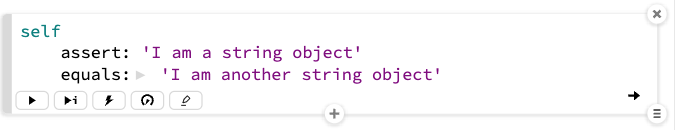
\includegraphics[width=\columnwidth]{stringComparisonSnippet}
  \caption{A failing string comparison assertion.}
  \label{fig:stringComparisonSnippet}
\end{figure}
In a normal setting, this assertion will fail, yielding a standard debugger view, as we see in \autoref{fig:genericDebugger}.
\steve{I wonder if the debugger view from Fig. 2 is really generic. I don't recognize it (not a critic), I think it is already a customized view. Are we seeing the source code of each method on the stack? Perhaps it would be more precise to specify "The generic GT debugger view with common standard debugging actions" (but I don't know).}
\begin{figure}[h]
  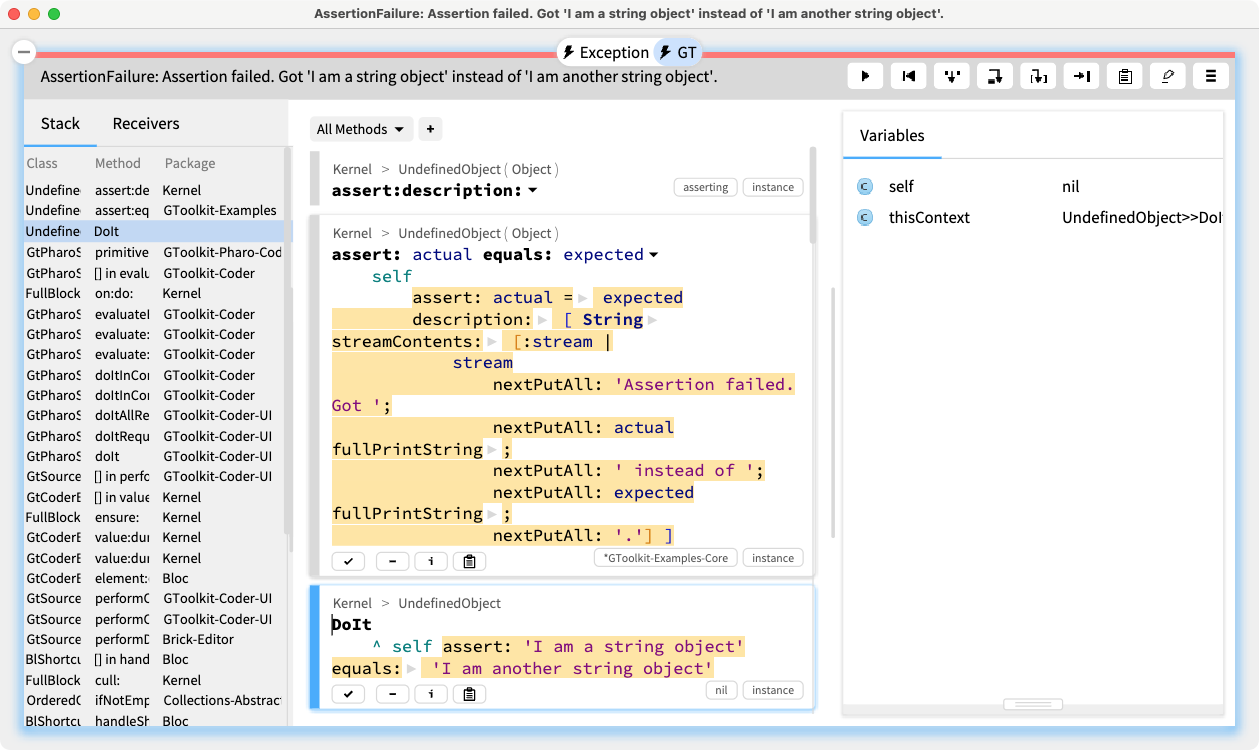
\includegraphics[width=\columnwidth]{genericDebugger}
  \caption{A generic debugger view.}
  \label{fig:genericDebugger}
\end{figure}
It will then take a developer some time to putter around in the debugger interface to understand the specific error (the strings do not match), and why the strings do not match.

Suppose that instead of seeing the generic debugger, we are offered a view that highlights the actual differences, as in \autoref{fig:stringComparisonView}.
\begin{figure}[h]
  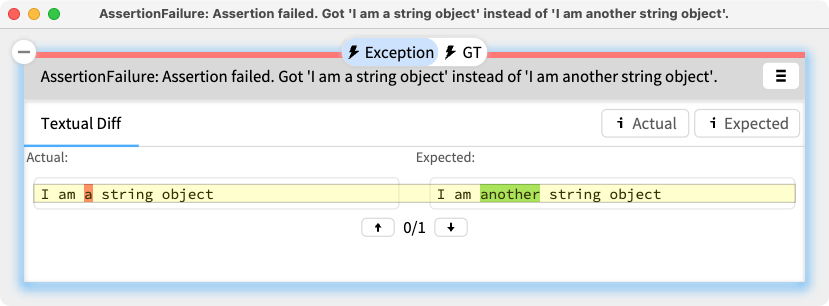
\includegraphics[width=\columnwidth]{stringComparisonView}
  \caption{A string diff debugger view.}
  \label{fig:stringComparisonView}
\end{figure}
Such a view not only homes directly in on the specific problem, but also highlights the individual differences in a dedicated ``diff'' view.
Furthermore, since the diff view already exists as a component used in other applications, the development effort is close to zero.

Moldable exceptions work as follows: when an exception is raised, the exception (an object) is caught and passed to the debugger.
Every exception not only provides the debugger with the context it needs to generate the debugging UI, but it can also offer alternative views and actions.
In the case of our implementation, this is achieved by the exception class providing specially annotated debugger extension methods.

This simple mechanism allows moldable exceptions to do three things:
\begin{enumerate}[(i)]
	\item provide domain-specific debugging views and actions,
	\item offer new debugger GUI interactions, and
	\item enable automated fixes (code transformations) for common programming errors.
\end{enumerate}

We will illustrate these three points with numerous examples.
\steve{Line 145 it does not seem correct that you present "numerous" examples. I did not count but I think you have some examples for each scenario. To me "numerous" implies "a lot", but my english is not that good --- like many reviewers ;)}
In \autoref{sec:inspectorViews} we introduce the \emph{moldable inspector}, which allows objects to define custom views when they are inspected.
In \autoref{sec:views} we show how custom debugger views can easily be defined in a similar way by adding simple annotated view methods to the class of a moldable exception.
In \autoref{sec:interactions} we show how a richer debugger interface can be provided in much the same way by leveraging existing GUI frameworks.
Finally we show an example of moldable exceptions enabling automated fixes in \autoref{sec:fixes}.
We summarize our contributions and discuss some possible future work in \autoref{sec:directions}, and we discuss related work in \autoref{sec:related}.
We conclude in \autoref{sec:conclusion}.

\ac{We could add maybe a section later describing a bit more the model. Moldable exceptions provide a list of debugging configurations used to create debuggers for that exception. A debugging configuration defines for example the pragmas used to find views and actions, but could also be different.}

% ============================================================
\section{The moldable inspector}\label{sec:inspectorViews}

Moldable exceptions build on and extend the notions of custom views and actions that can be used to extend a \emph{moldable object inspector}~\cite{Chis15a}.
When a moldable object inspector is opened on an object it looks for any view methods defined in the class of that object, and uses those methods to create custom views.

Let us consider a typical example.
Suppose we have an implementation of a Ludo\footnote{A simple game in which players move tokens around a board based on the roll of a die.
\url{https://en.wikipedia.org/wiki/Ludo}} game.
Players alternate in throwing a die and moving a token until one player reaches their goal square.
In \autoref{fig:ludoRawBoardViews} we see at the left the classical \emph{Raw} view supported by a typical object inspector.
\begin{figure}[h]
  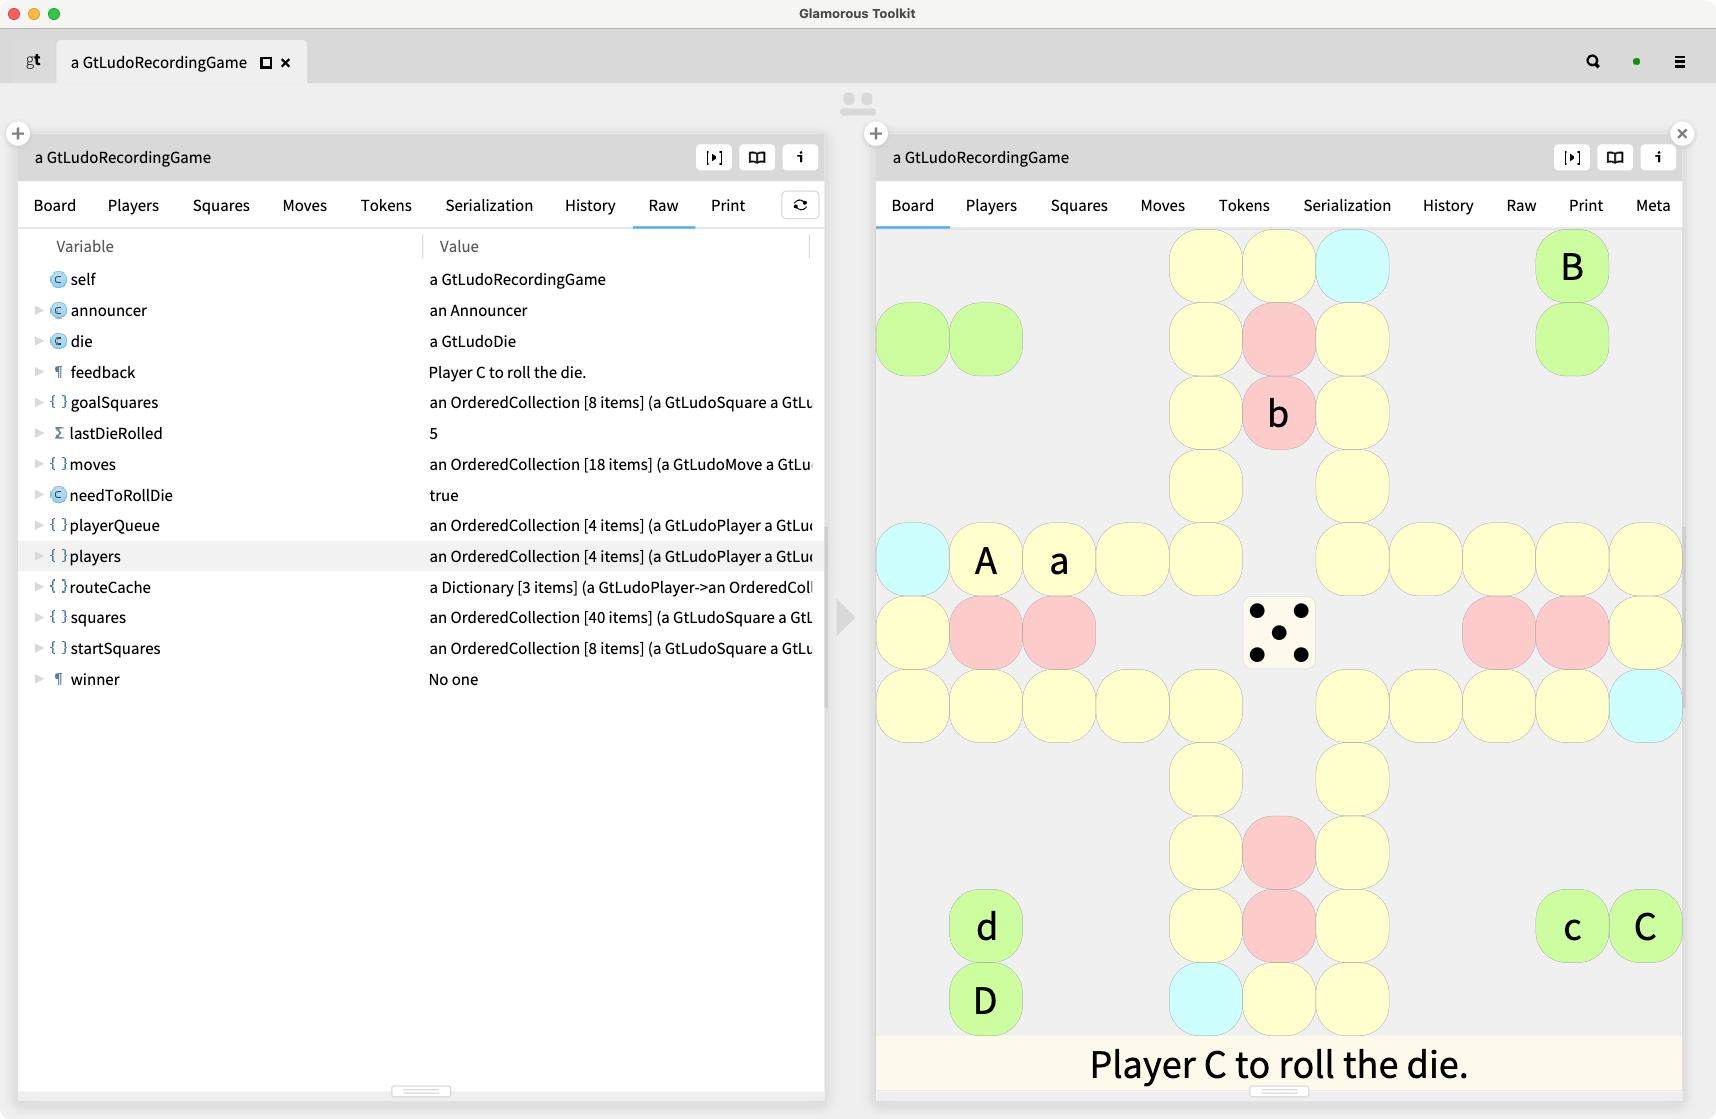
\includegraphics[width=\columnwidth]{ludoRawBoardViews}
  \caption{A classical raw view of a Ludo game next to a graphical \emph{Board} view.}
  \label{fig:ludoRawBoardViews}
\end{figure}
It just shows the state of the object as a list of instance variables and their values.
At the right, however, we see an alternative, graphical \emph{Board} view showing the current state of the game as a user would see it.

In general, a variety of views may be more useful than the classical``raw'' view, and this is also true for the Ludo game.
In \autoref{fig:ludoMovesMoveViews} we see a \emph{Moves} view that lists all the moves of the game played thus far.
\begin{figure}[h]
  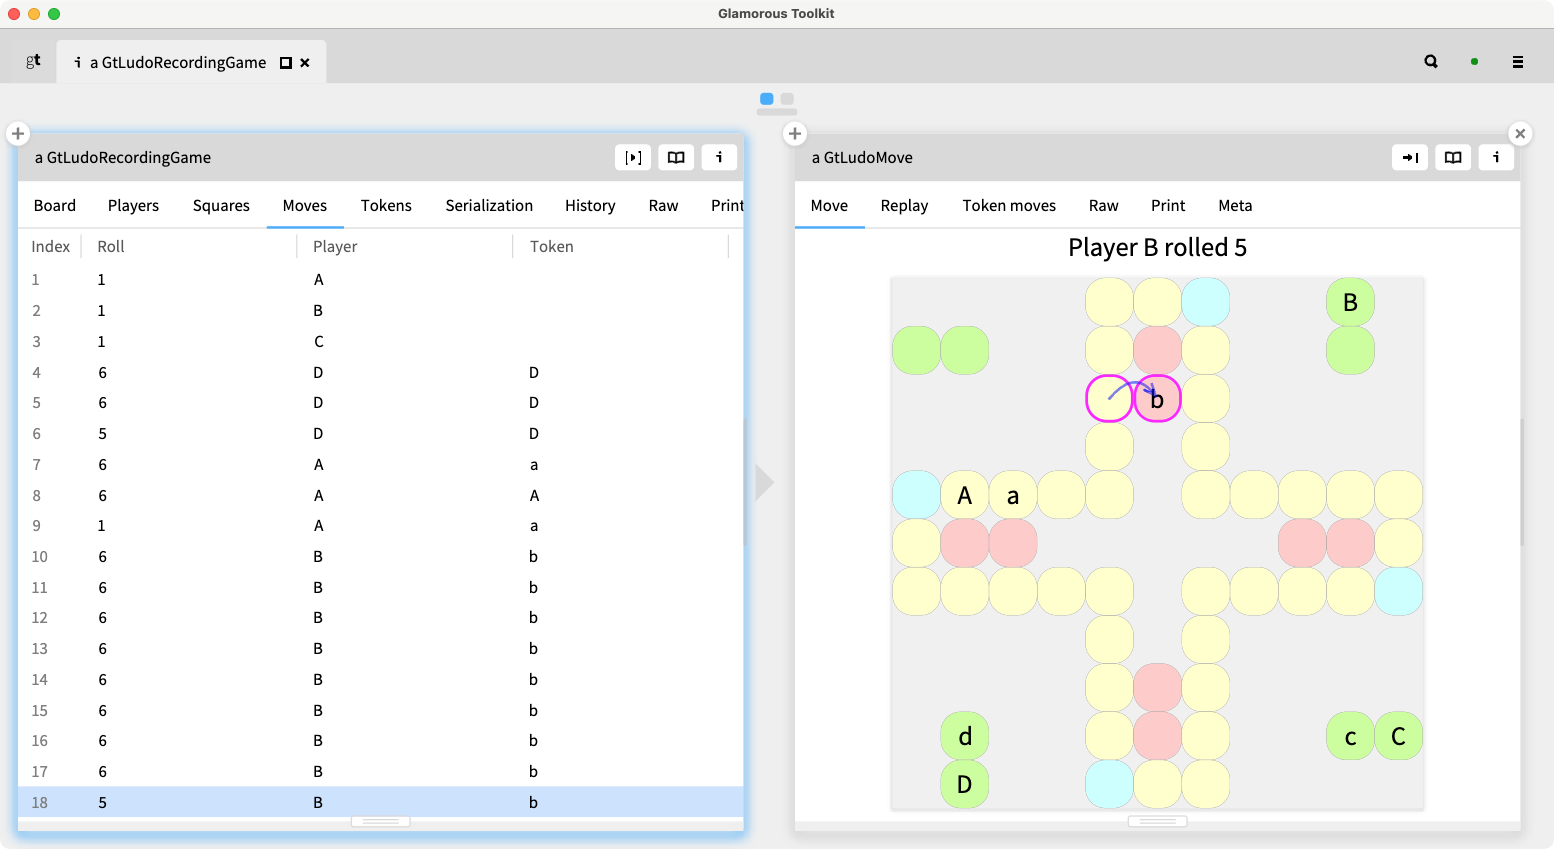
\includegraphics[width=\columnwidth]{ludoMovesMoveViews}
  \caption{A custom historical \emph{Moves} view ofa Ludo game, and a custom graphical view of a selected move.}
  \label{fig:ludoMovesMoveViews}
\end{figure}
By clicking on a move (at the left) you can then inspect (at the right) the corresponding \st{GtLudoMove} object, with its custom views, in this case showing the details of what happened in this move.

In \autoref{fig:ludoMovesSource} we see the source code defining the \emph{Moves} view.
\begin{figure}[h]
  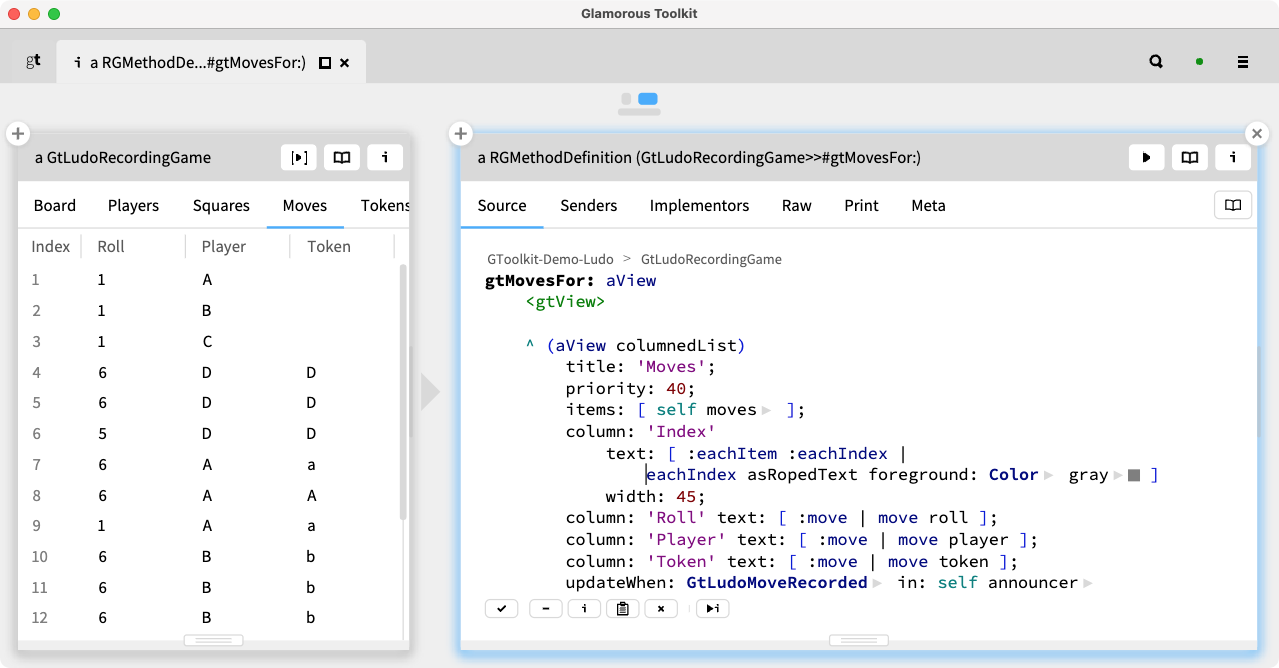
\includegraphics[width=\columnwidth]{ludoMovesSource}
  \caption{The \emph{Moves} view next to its source code.}
  \label{fig:ludoMovesSource}
\end{figure}
This method uses just a few lines of code to create a browsable ``columned'' list of past moves with several columns for the details of each move.
View methods are recognized by the moldable inspector through a dedicated annotation, in exactly the same way that a test runner tool in a classical IDE recognizes Java test case methods because they are tagged with a \st{@Test} annotation.
In this case the annotation is \st{<gtView>}, seen in the second line of the method.

% ============================================================
\section{Adding custom debugger views}\label{sec:views}

Moldable exceptions provide custom debugger views and actions in essentially the same way as the moldable inspector.
Moldable exceptions are instances of an \emph{Exception} class that has been extended with a dedicated method for each custom debugger view or action.
These methods are annotated with a \lst{<gtExceptionView>} pragma.

Let us consider that the Ludo game has been implemented with the help of \emph{Design by Contract}~\cite{Meye92b}.
Rolling a die when a player should move, or vice versa, constitutes a precondition violation, which raises a \st{LudoMoveAssertionFailure}.
Similarly, if an attempt is made to move the wrong player's token, this will trigger a precondition failure.
\begin{figure}[h]
  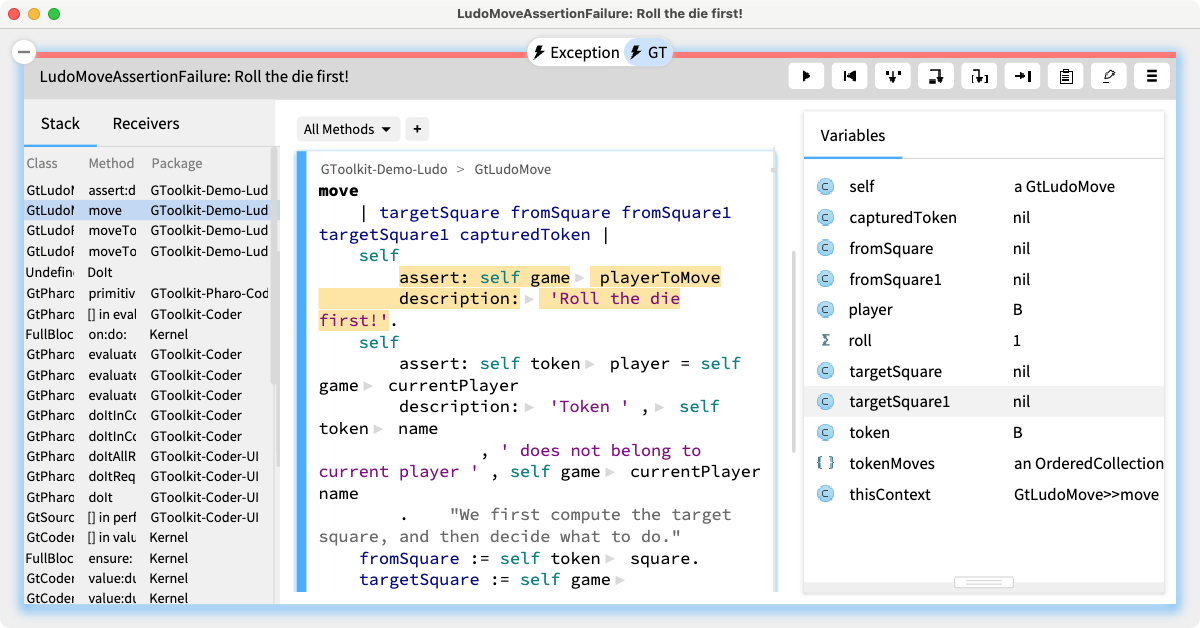
\includegraphics[width=\columnwidth]{ludoClassicDebugger}
  \caption{A classical debugger for a precondition failure.}
  \label{fig:ludoClassicDebugger}
\end{figure}
Normally, this would fire up the classical debugger, as seen in \autoref{fig:ludoClassicDebugger}.
Although the precondition violation is clearly reported, the debugger interface is not ideal for tracking down the actual reason for the violation.

What we would perhaps like to see instead is the current state of the game, in addition to a history of the past moves.
We could possibly find these by navigating through the existing debugger views, but why not show them directly?
After all, we know that whenever this exception is raised, what it is that we would like to see.
Furthermore, if we already have such views defined elsewhere (we do!), it is not a question of defining new views, but of reusing them in the context of the debugger.
We just need to define two new view methods in the class \lmaf.

Here is the definition of the first view, which simply forwards (delegates) the view to another existing one.
\steve{Why, in the script from line 250, the method does not have a `<gtView>` pragma while the one from line 325 does? I would suggest removing the `<gtView>` pragma since it is not explained and it does not serve the explanations of the idea.}
\begin{code}
gtGameViewFor: aView
	<gtExceptionView>
	^ aView forward
		title: 'Game';
		priority: 10;
		object: [ move game ];
		view: #gtPositionsFor:
\end{code}
\steve{I do not understand the result of the priority "10" in line 254 when I look at the screenshot. Perhaps change it to priority "1"?}

Let us step through the code: \st{gtGameViewFor:} is the name of the view method, which takes as its argument \st{aView}, the view to be defined.
The method is annotated with \lst{<gtExceptionView>}, which tells the moldable debugger to enable the view whenever \lmaf is raised.
We return (\st{^}) the result of sending \st{forward} to \st{aView}, giving the view a title and a priority (order in which views) appear, and we specify the object to forward to (the move's \st{game}) and the already existing view method to forward to (\st{gtPositionsFor:}).

We similarly define a method for the history of past moves, and now the debugger, instead of showing us the classical debugger, will offer us the two views seen in \autoref{fig:ludoCustomViews}.
\begin{figure}[h]
  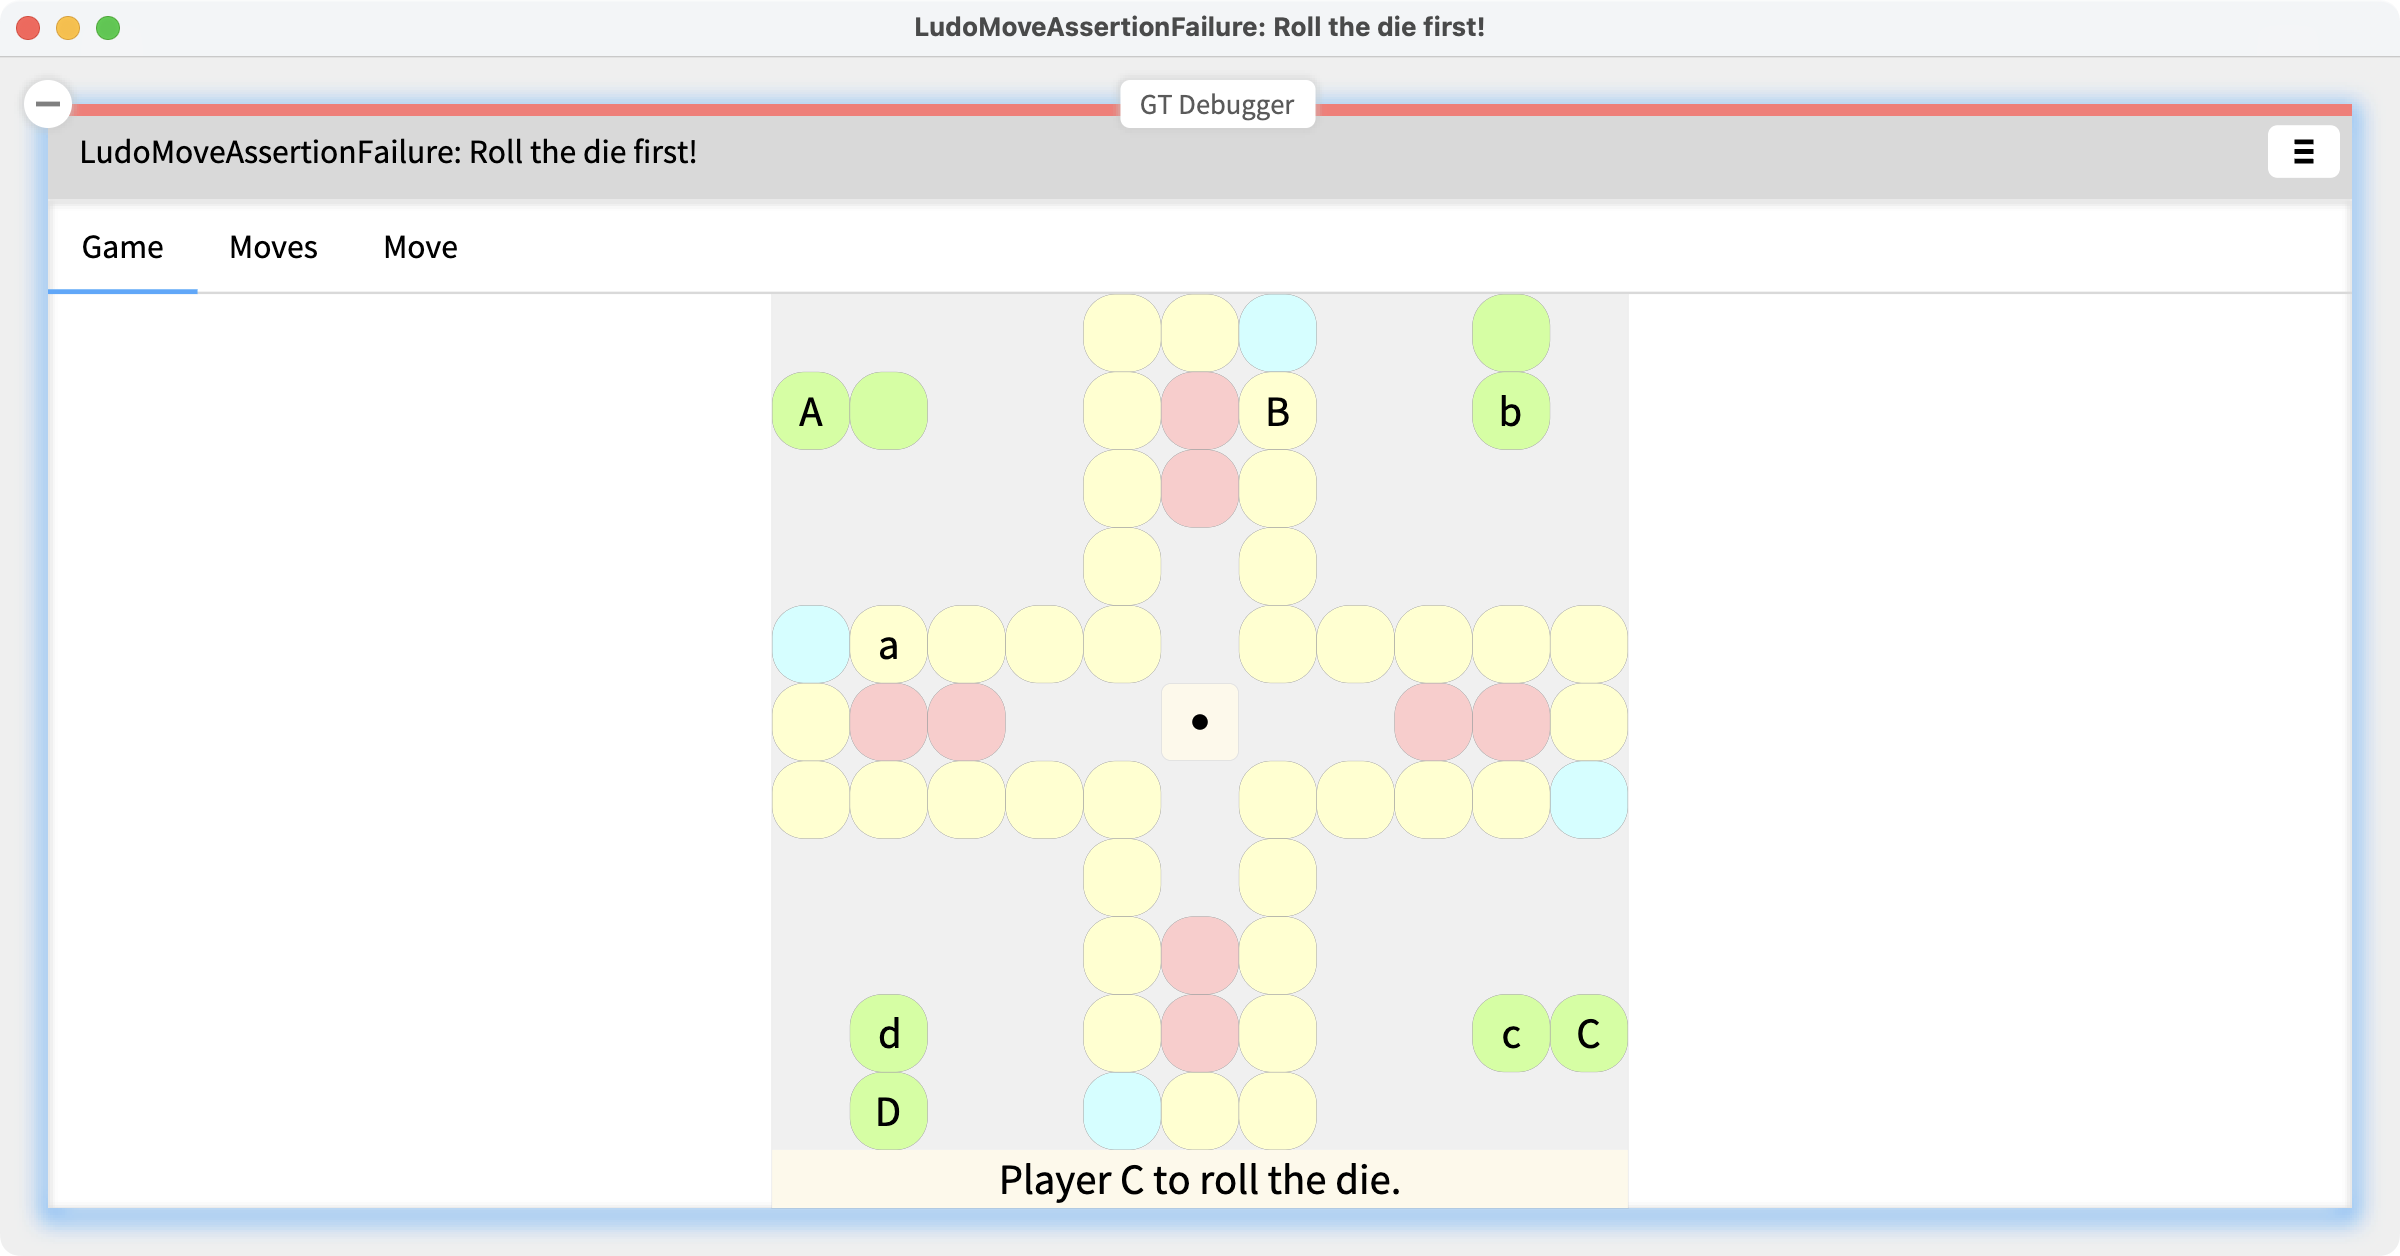
\includegraphics[width=\columnwidth]{ludoView1-Game}
  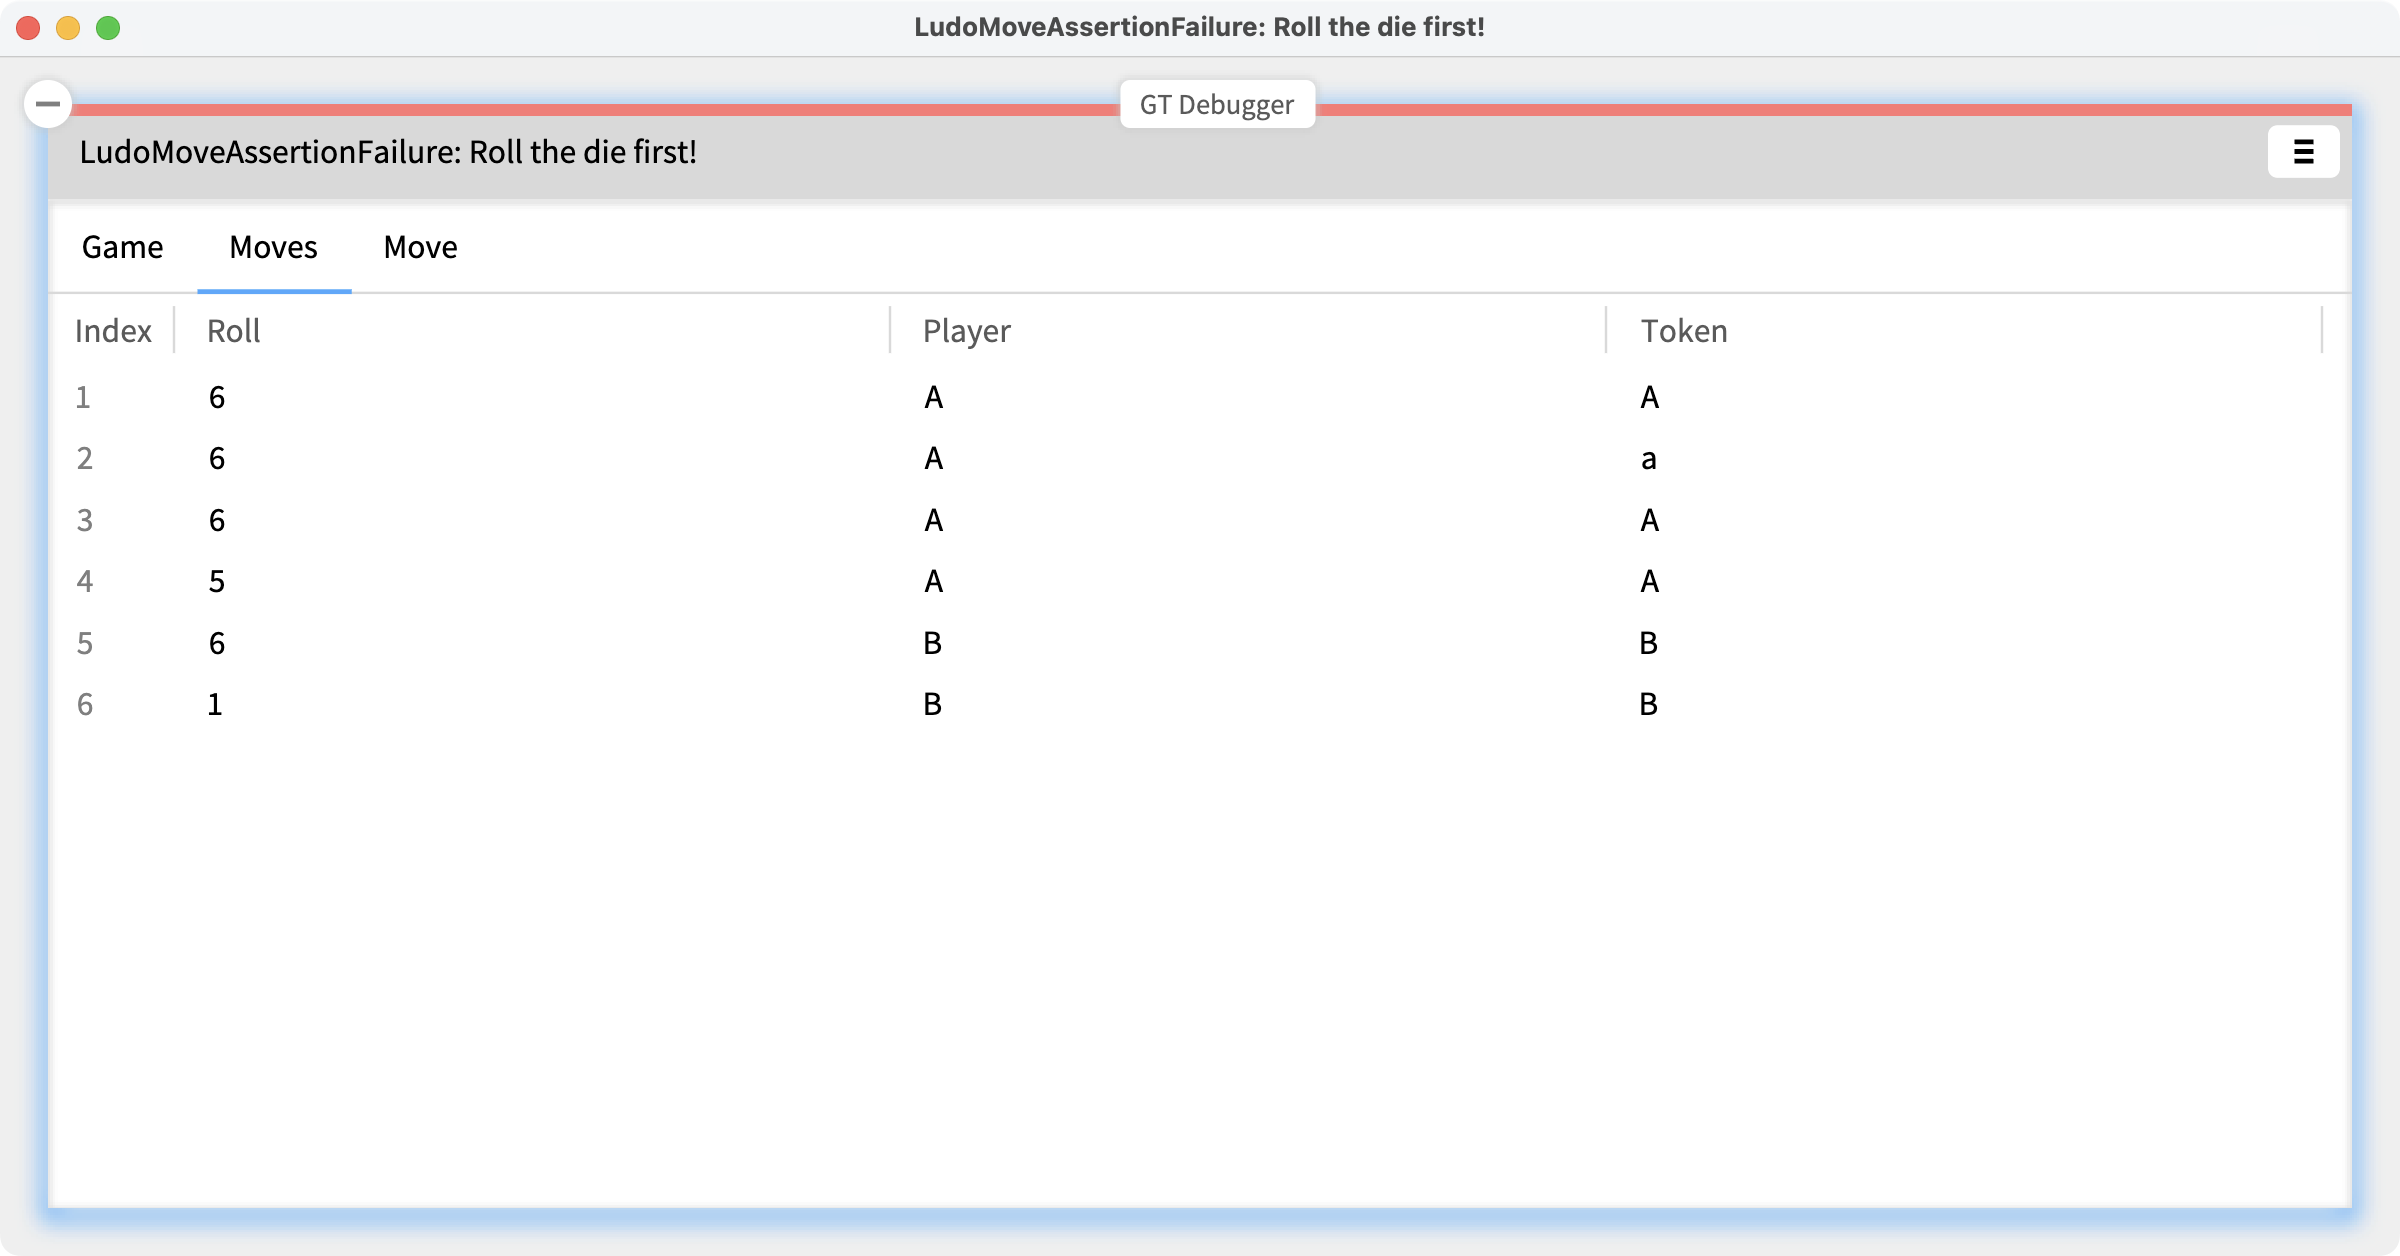
\includegraphics[width=\columnwidth]{ludoView2-Moves}
  \caption{Custom debugger views for the Ludo game.}
  \label{fig:ludoCustomViews}
\end{figure}
The Game view shows us the current game state graphically, and the Moves view shows us a browsable list of past moves.
Note that we can always switch to the standard debugger by selecting the \emph{GT} button at the top.
%\ab{Line 273: "the old debugger" => "the standard debugger"}
%\steve{line 273 "old debugger" -> "standard debugger" I think that in many cases customized debugger views might come as complement to the standard debugger. Since there can sometimes be no dedicated actions in views, they can serve as additional visualization tools to find and understand data that helps taking a decision in the standard debugger.}

The \emph{Moves} debugger view is also defined by reusing the existing object inspector \emph{Moves} view:
\begin{code}
gtMovesViewFor: aView
	<gtExceptionView>
	^ aView forward
		title: 'Moves';
		priority: 20;
		object: [ move game ];
		view: #gtMovesFor:
\end{code}

The assertion diff debugger view we saw earlier in \autoref{fig:stringComparisonView} is similarly defined as a method of \st{AssertionFailure}.
\begin{code}
AssertionFailure>>gtTwoPanesStringDiffFor: aView
	<gtView>
	<gtExceptionDebuggingView>
	| assertionContext |
	self gtHasStack ifFalse: [ ^ aView empty ].
	assertionContext := self gtLocateAssertEqualsContextWithComparableTypes.
	assertionContext ifNil: [ ^ aView empty ].
	^ aView forward
		title: 'Textual Diff';
		priority: 0;
		object: [ assertionContext ];
		view: #gtTwoPanesStringDiffFor:
\end{code}
The key difference is that not every \st{AssertionFailure} is raised as the result of a comparison.
For this reason, in lines $6-7$, the view will be suppressed (\st{^ aView empty}) in case the assertion did \emph{not} fail in the context of an \st{assert:equals:} check.

% ============================================================
\section{Providing domain-specific debugger interfaces}\label{sec:interactions}

\ab{Section 3 is difficult to read. I am not sure what exactly you mean by "domain-specific debugger interface" actually. Are we talking about user-interface?}

\steve{By "interfaces" (line 345) do you mean "Human Machine Interfaces" or just views? I understand it is just views, because there are no actions visible in the example and it follows the previous sections where you reused views and here you create new ones. In that case I suggest keeping the vocabulary consistent because HMI = views + actions + user experience design, while here it is only a view. I think also the title section could be stronger: you are actually "building" rather than "providing" debugger views. Perhaps changing the title to "Building domain-specific debugger views"? (it would be consistent with the previous section)}

The examples we have seen so far have reused existing inspector views, but sometimes there is a need to develop a new kind of debugger interface.
This also does not necessarily imply a heavy implementation effort.

Let us consider the case of assertion errors being raised while testing a user interface interaction with the help of a GUI ``Scripter'' object.
\ac{We could add one paragraph describing scripter, and why we need it.}
We introduce three dedicated debugger views.
The \emph{Scripter preview} (\autoref{fig:scripterPreview}) shows the result of a scripted interaction:
\ab{Line 354: I do not follow the link between the scripter preview and the previous Ludo example. Why a notebook page has been created?}
\begin{figure}[h]
  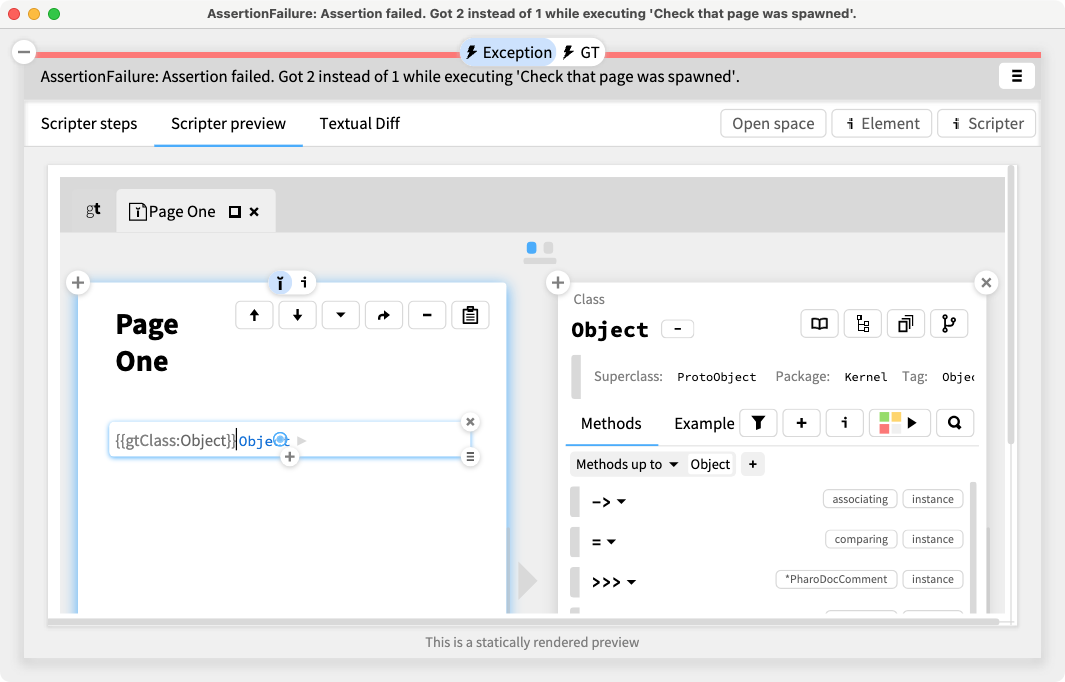
\includegraphics[width=\columnwidth]{scripterPreview}
  \caption{Scripter preview.}
  \label{fig:scripterPreview}
\end{figure}
\begin{inparaenum}[(i)]
	\item a notebook page has been created, containing a link to the class \st{Object}, and
	\item the link to the class has been clicked, opening a source code browser on the class.
\end{inparaenum}

The \emph{Scripter steps} view (\autoref{fig:scripterStepsViewClicked}) shows us a graphical tree view of the steps performed by the GUI Scripter, as well as the assertions that have been checked.
\ab{Line 374: What the graphical tree view is about?}
\begin{figure}[h]
  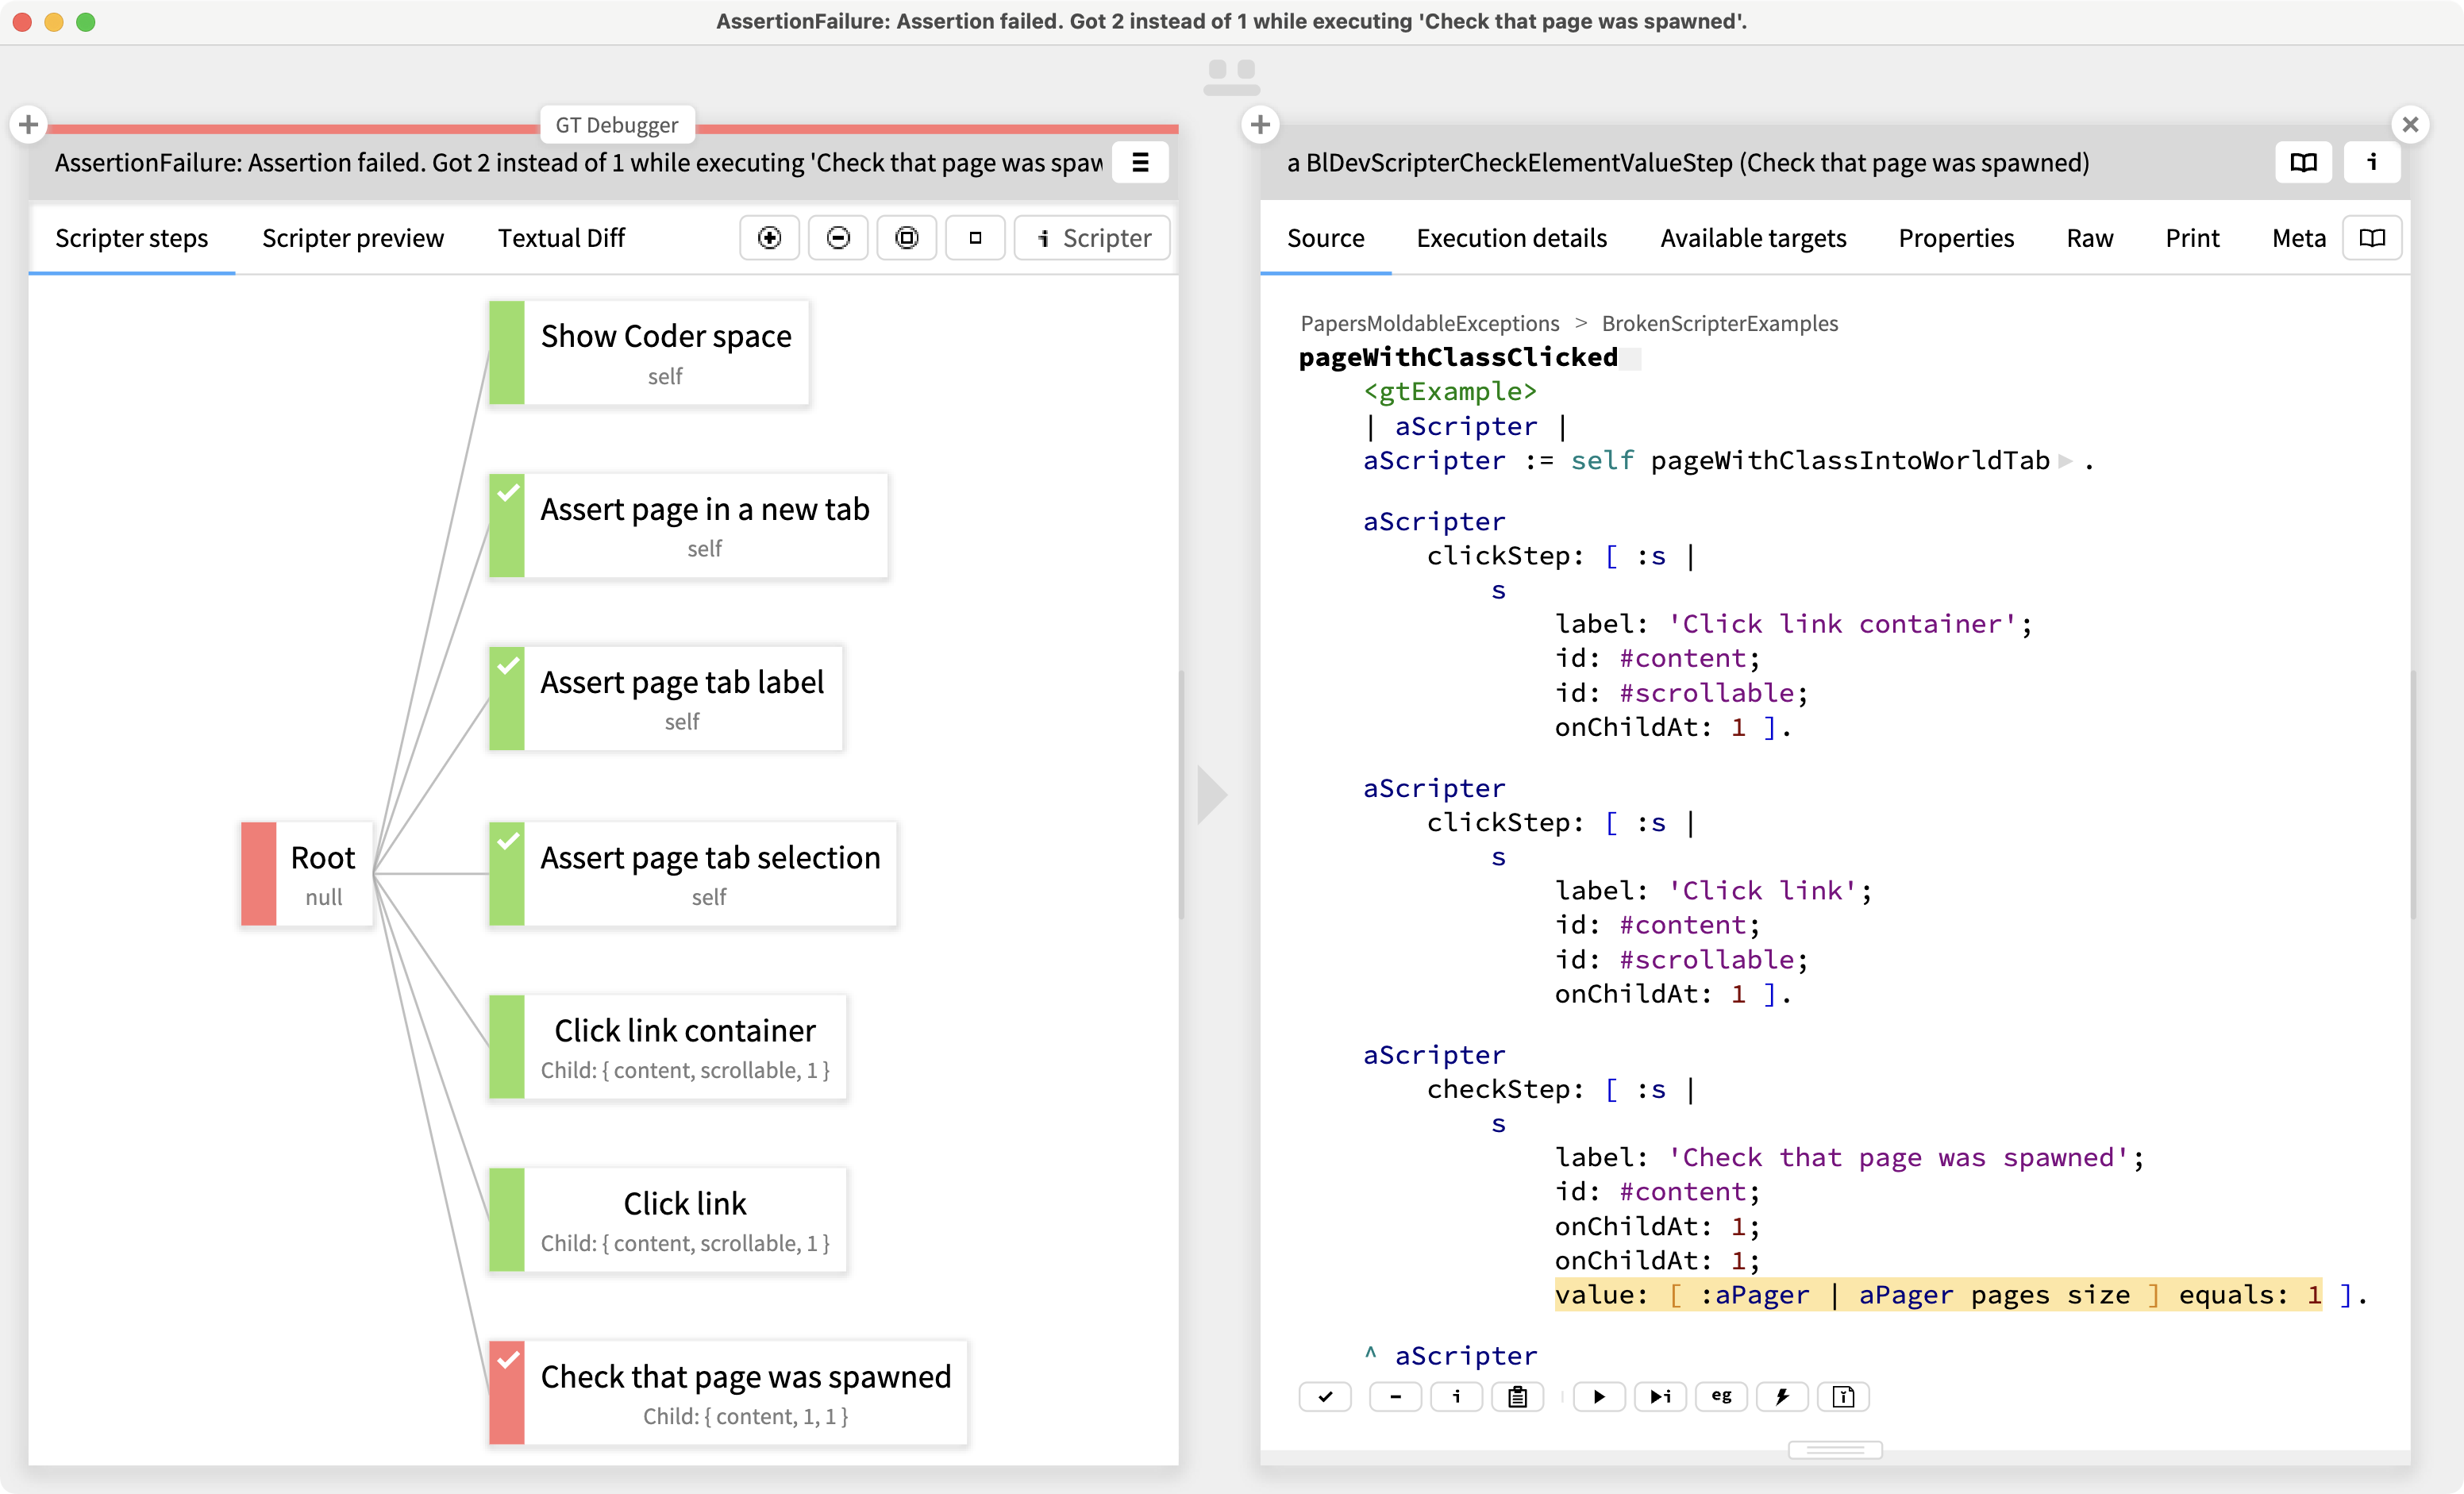
\includegraphics[width=\columnwidth]{scripterStepsViewClicked}
  \caption{Scripter steps view.}
  \label{fig:scripterStepsViewClicked}
\end{figure}
The green steps and assertions have succeeded, whereas the red ones have failed.
By clicking on any step or assertion node, we can see the corresponding code highlighted in the scripter method at the right.

Finally, the \emph{Textual Diff} view (\autoref{fig:scripterDiff}) is the same one we have seen earlier, reused again.
\begin{figure}[h]
  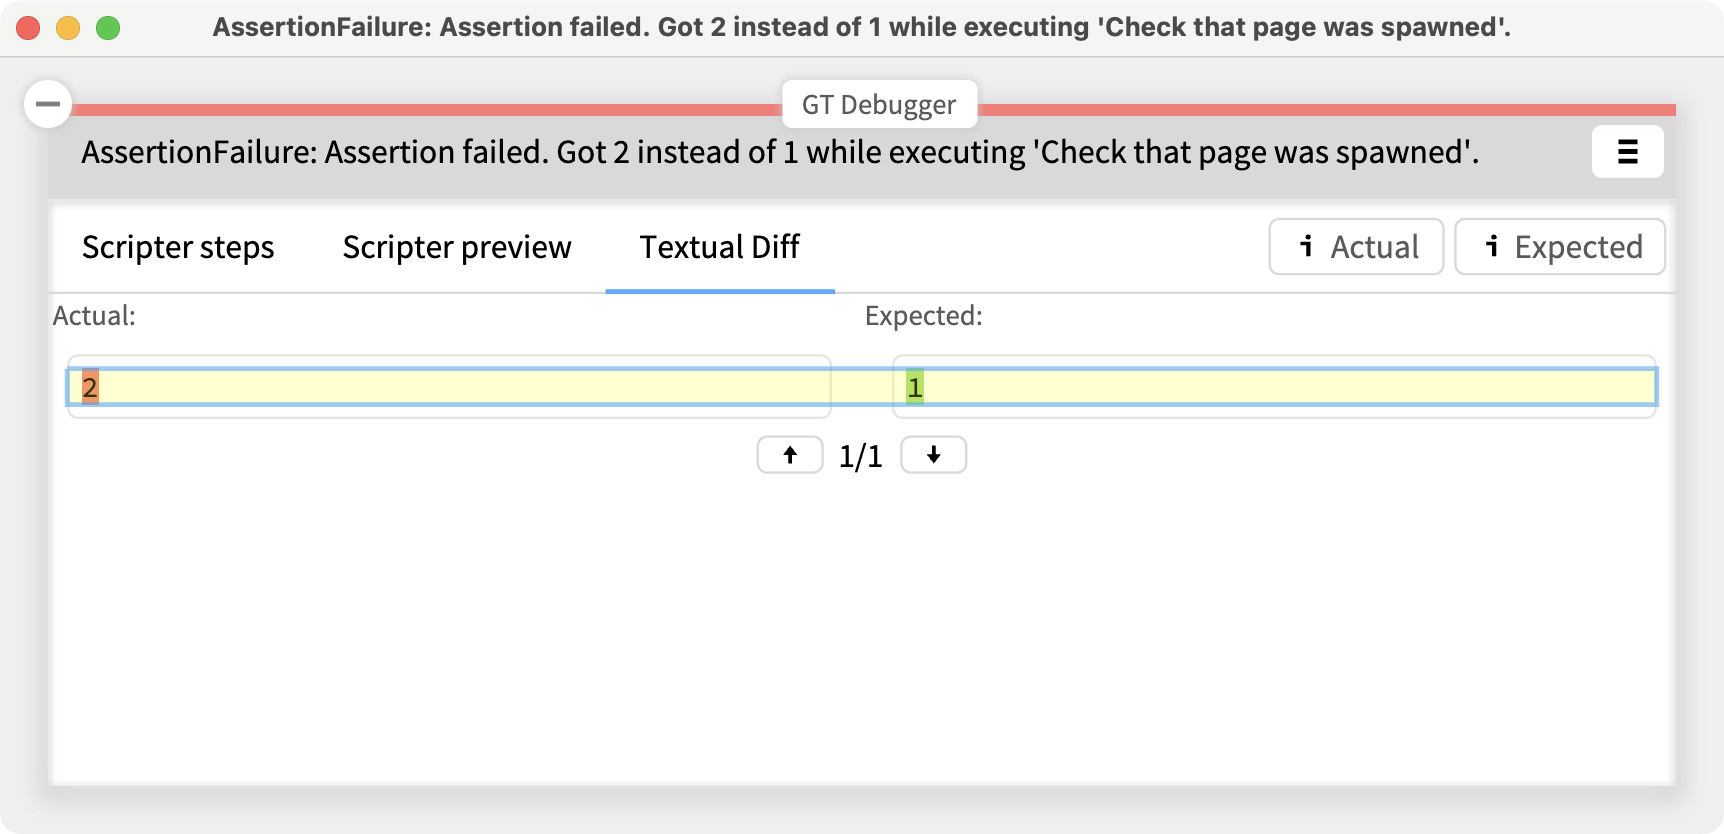
\includegraphics[width=\columnwidth]{scripterDiff}
  \caption{Scripter textual diff view.}
  \label{fig:scripterDiff}
\end{figure}
It just tells us that the check should verify that there are now two pages in the pager, not just one, as we can also see in the \emph{Scripter preview}.

\paragraph{Why do we need these views?}
The problem with the standard debugger is that, due to the way the GUI Scripter schedules the steps, the offending method (\ie the \lst{page\-With\-Class\-Clicked} method we see in \autoref{fig:scripterStepsViewClicked}) is \emph{not on the stack} (\autoref{fig:scripterClassicDebugger}) at the point where the exception is raised.
\begin{figure}[h]
  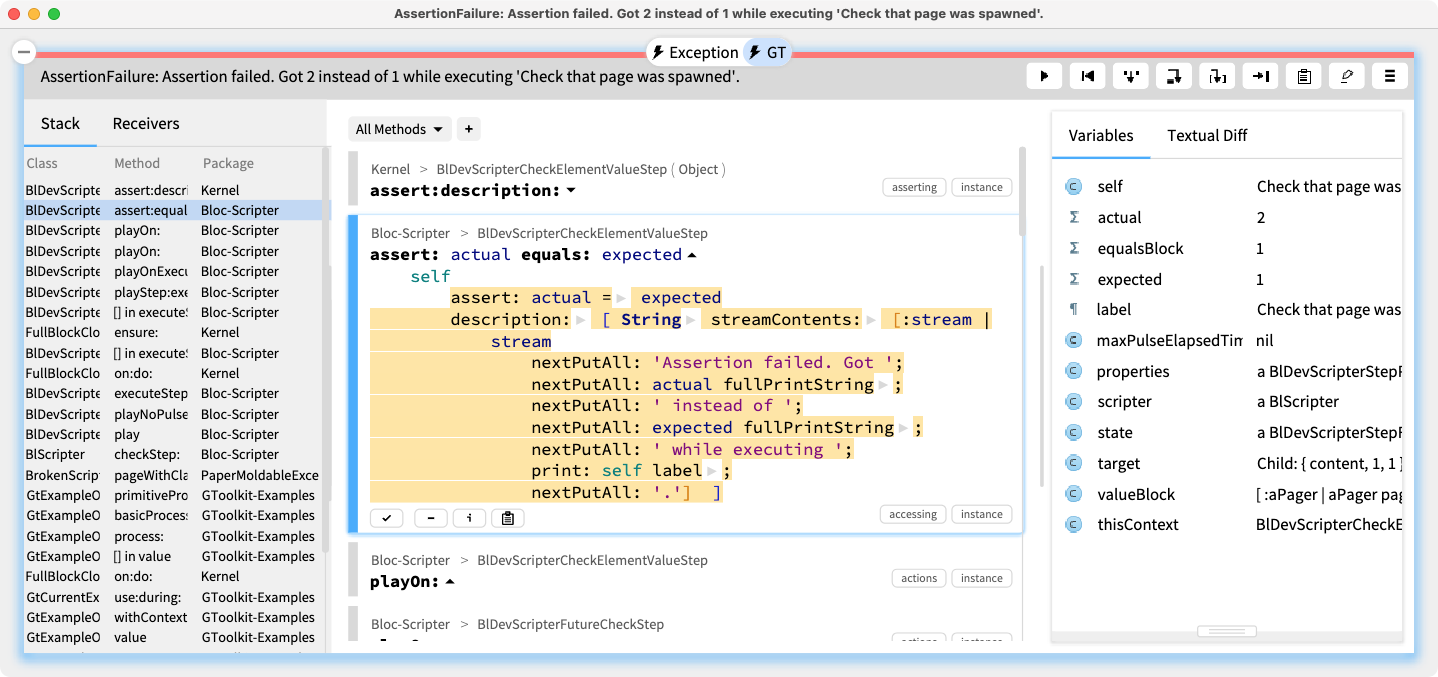
\includegraphics[width=\columnwidth]{scripterClassicDebugger}
  \caption{The trouble with the standard debugger.}
  \label{fig:scripterClassicDebugger}
\end{figure}
Although it is possible to get at the information we seek, it is clumsy, and the classical stack view only confuses matters instead of helping us to debug the problem.
This can be the case with many application domains, especially those that depend on event scheduling.
The run-time stack does not do a good job of telling you how the events have been triggered, so another kind of view is needed.
\steve{line 435 you say that the "run-time stack does not do a good job telling you how the events have been triggered". Perhaps worth adding that it is because it provides a generic view over the execution of any program, while you are in need of a view providing very specific information.}

\paragraph{How hard is it to implement a domain-specific debugger interface?}
\steve{line 438 you ask "How hard is it to implement a domain-specific debugging interface?" -> I feel like this paragraph misses some comparison with how difficult it would be to do it with a standard debugger. That particular point is not covered in the related work either. For instance, with Pharo (before we implemented a similar moldable exception mechanism after Andrei explained to us, even if much less moldable than GT on the view part), we literally would have to implement a new debugger, probably by subclassing the existing one, having to deal with complex implementation problems to integrate a specific view, and then we would have to know when to choose the standard debugger and when to choose that specific one. Worse, if we use the specific one, and if we encounter another problem (imagine a DNU), since that debugger is specific to the example it would not be able to handle the DNU and allow me to debug it. This means extra implementation logic to handle such case... so tedious... }
The \emph{Scripter steps view} is implemented using a version of \emph{Mondrian}~\cite{Pena13b,Meye06a}, a builder for graph-based visualizations.
In \autoref{fig:scripterStepsViewSource} we can see the entire source code of the view expanded in place, implemented in just four methods.
\begin{figure}[h]
  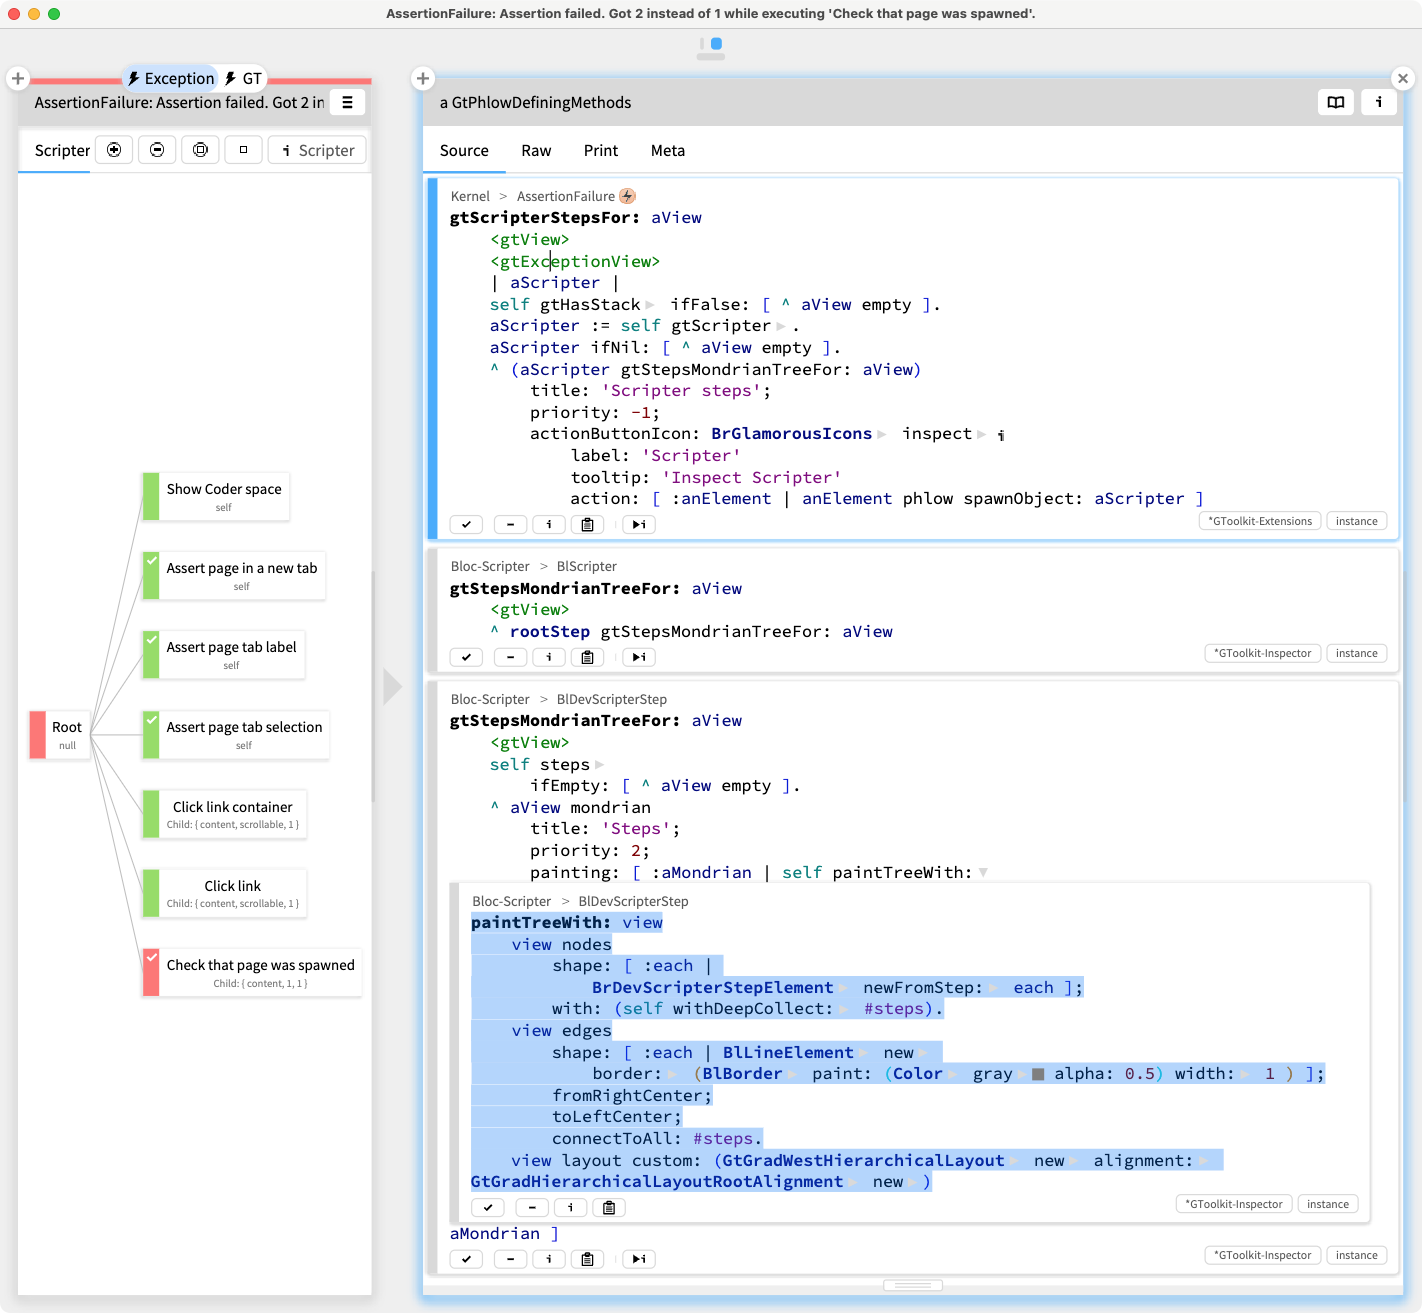
\includegraphics[width=\columnwidth]{scripterStepsViewSource}
  \caption{The Scripter steps source code.}
  \label{fig:scripterStepsViewSource}
\end{figure}
\steve{Just thinking now about the screenshots: they are small and we can't read much of the code. I understand that might not be that important such as in Fig. 12 where the point is showing the short amount of lines of code. It is however frustrating for the reader that cannot not see that there is code :P but I don't know what you can do there...}\on{Gave more space to the source code.}
The debugging view at the top just adds a ``Inspect Scripter'' button to the next method, an object inspector view for a Scripter.
This in turn just delegates to the \emph{Steps} view of a \st{BlDevScripterStep} object.
Finally, this method embeds a Mondrian visualization implemented in 12 lines of code in the \st{paintTreeWith:} method.

% 14 LOC AssertionFailure>>#gtScripterStepsFor:
%  3 LOC BlScripter>>#gtStepsMondrianTreeFor:
%  8 LOC BlDevScripterStep>>#gtStepsMondrianTreeFor:
% 12 LOC BlDevScripterStep>>#paintTreeWith:
% TOTAL: 12 mondrian + 25 boilerplate

Obviously this does not prove that all domain-specific debugger interfaces will be so tiny, but it does demonstrate that a useful debugger extension can be implemented in an almost trivial amount of code.

% ============================================================
\section{Enabling automated fixes}\label{sec:fixes}

Many cases of common programming errors can be automatically repaired.
A good example is that of deprecated methods for which a well-defined alternative is available.
In Pharo Smalltalk this is achieved with the \lst{\#de\-pre\-cat\-ed:trans\-form\-With:} message defined in the class \st{Object}~\cite{Duca22a}.
% \ac{We can cite and compare with Duca22a.}
It takes as arguments
\begin{inparaenum}[(i)]
	\item an explanatory string, and
	\item a source code transformation rule.
\end{inparaenum}    
We see an example below, where the method \st{ClassDescription>>definition} has been deprecated, and should be replaced by \st{definitionString} in client code.
\begin{code}
ClassDescription>>definition
	"Answer a String that defines the receiver."
	self
		deprecated: #definition
		transformWith: '`@receiver definition' -> '`@receiver definitionString'.
	^ self definitionString
\end{code}
While the \st{deprecated:} message normally spawns a Debugger, when a transformation rule is supplied, instead the client code is automatically rewritten, after which execution proceeds.
Here the transformation rule matches a send of \st{definition} for some receiver expression, and rewrites the message send to \st{definitionString}.

The fix is so straightforward, that it can be applied without any programmer intervention, or the need to spawn a debugger.
In \autoref{fig:deprecationDemo} we see the result of running client code of the old, deprecated method.
\begin{figure}[h]
  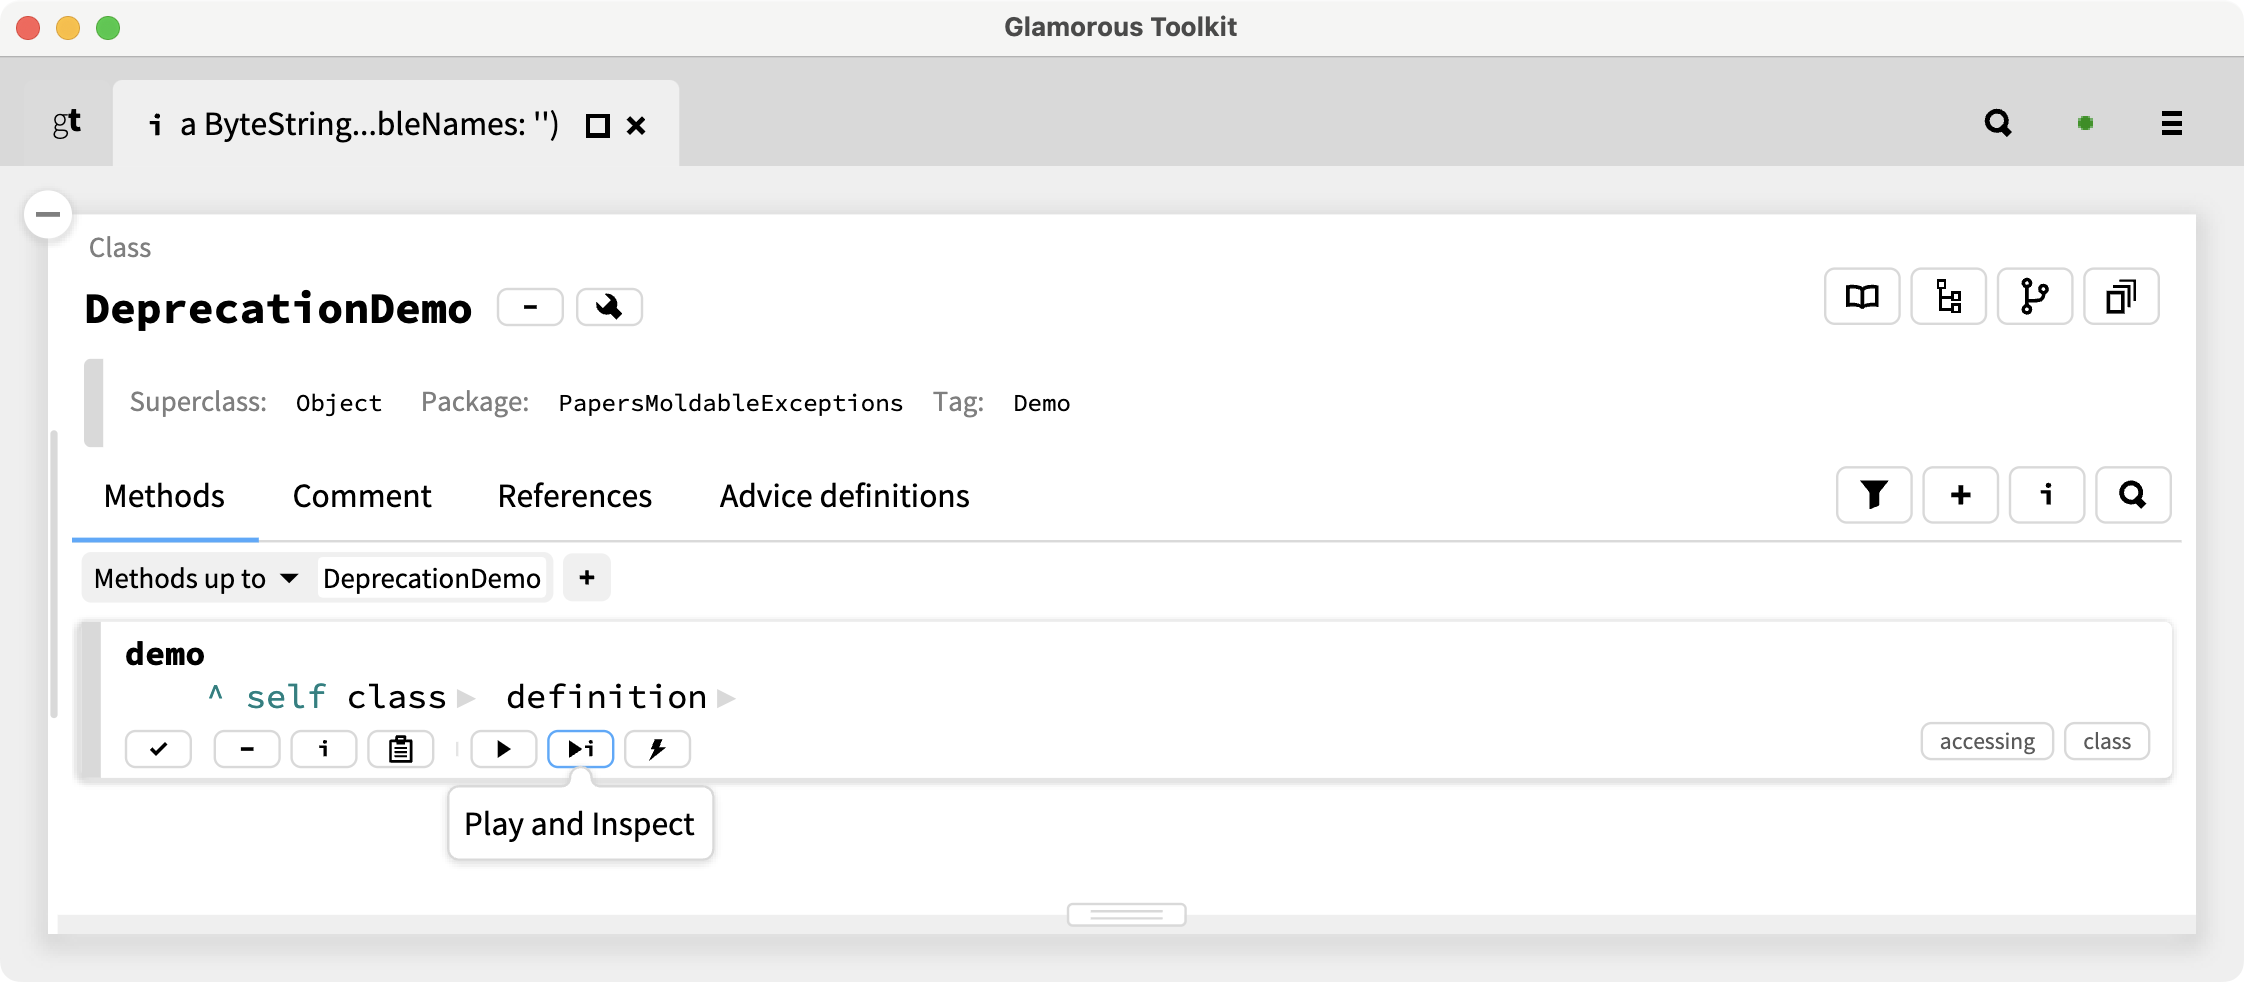
\includegraphics[width=\columnwidth]{deprecationDemoBefore}
  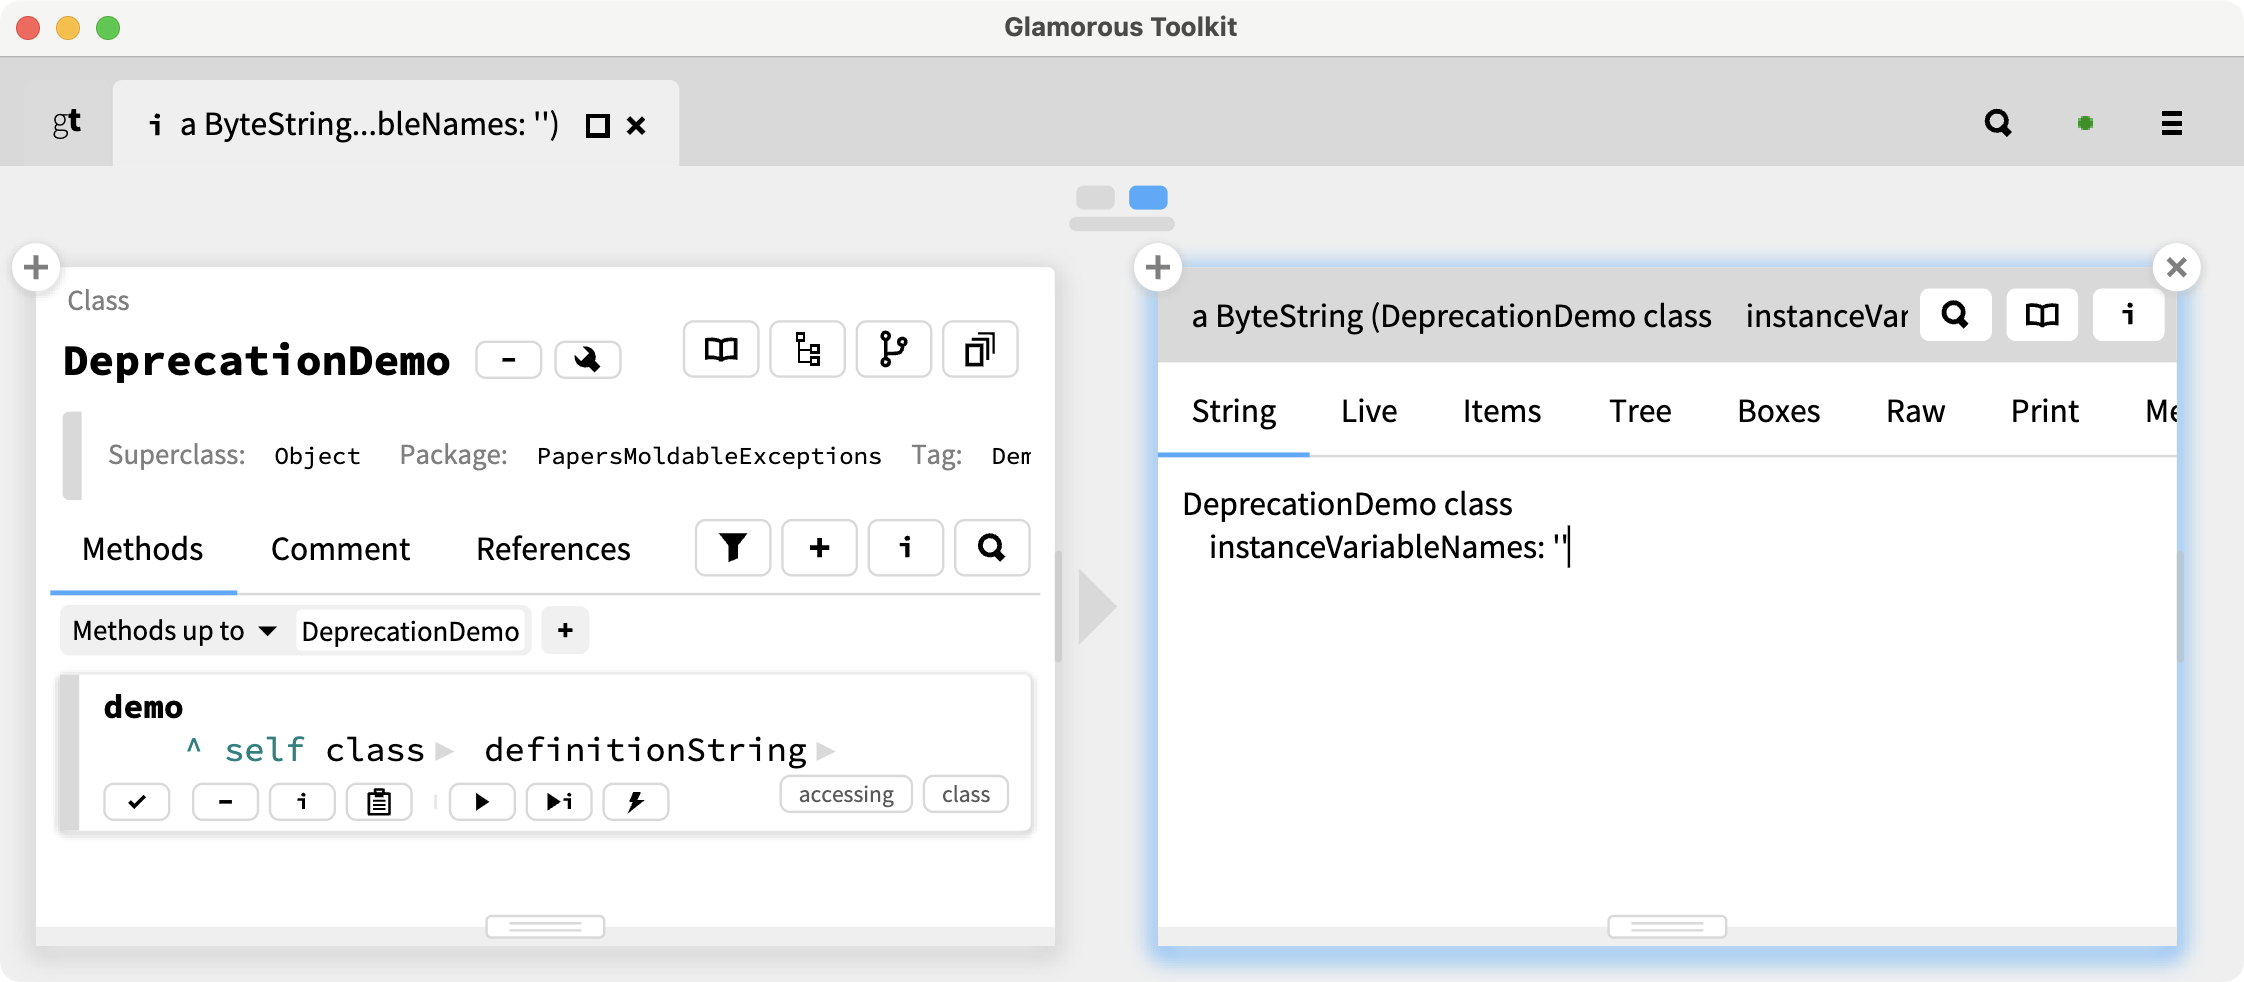
\includegraphics[width=\columnwidth]{deprecationDemoAfter}
  \caption{Automatically rewriting a client of deprecated code, before and after execution.}
  \label{fig:deprecationDemo}
\end{figure}
If we \emph{Play and Inspect} the method, we see that it is rewritten, and then directly evaluated.

Unfortunately the automated fix for deprecated methods is bespoke behavior.
Pharo offers no general mechanism for automatically fixing other kinds of simple programming errors.
Moldable exceptions, however, offer a more general solution.

Consider the case of a common programming error being that of providing to an API an object of the wrong type, or of the right type but the wrong state.
While the first kind of mistake could arguably be caught a static type system, detecting objects being in a wrong state is rather a run-time issue, typically caught by a precondition.
Some common cases can be fixed by rewriting the client code.
In \autoref{fig:emptyViewError} we see the source code for a custom inspector view that incorrectly returns \st{aView} instead of \st{aView empty} in the preamble.
\begin{figure}[h]
  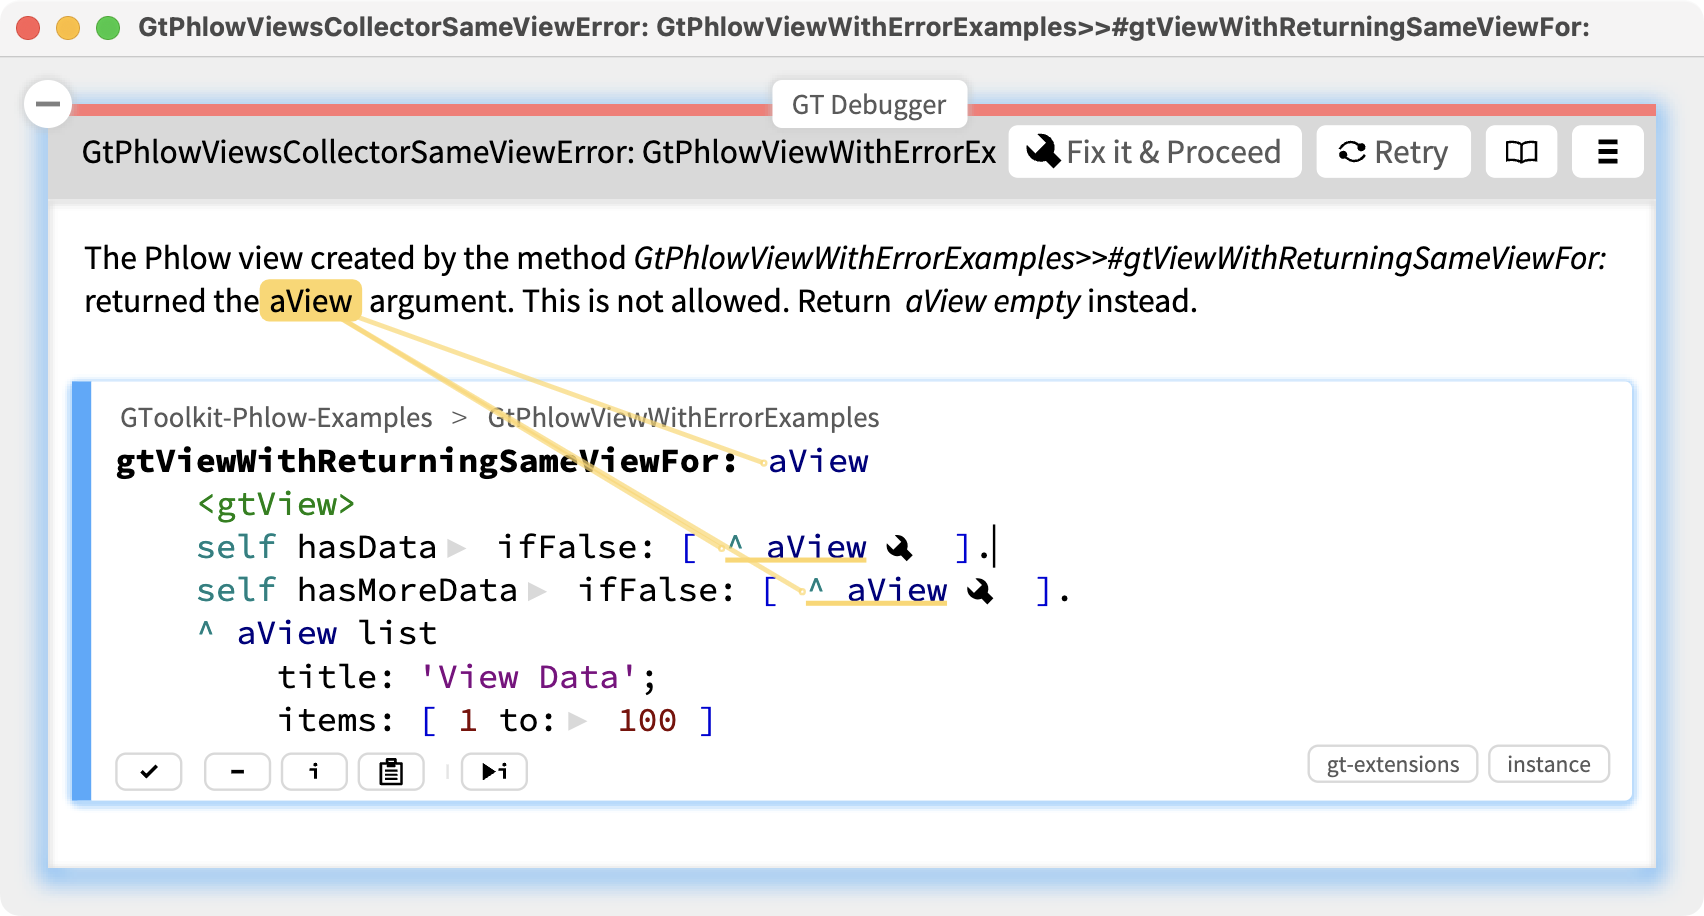
\includegraphics[width=\columnwidth]{emptyViewError}
  \caption{Catching an ``empty view'' error.}
  \label{fig:emptyViewError}
\end{figure}
This custom debugger view decorates the source code with an explanation pointing out the likely errors.

Since such preambles are a common idiom in defining GT inspector views, and the error is also not uncommon, it becomes easy to fix with the help of a transformation.
\autoref{fig:emptyViewErrorFix} shows the result of performing the \emph{Fix it \& Proceed} action: a refactoring widget is generated that proposes a code transformation.
\begin{figure}[h]
  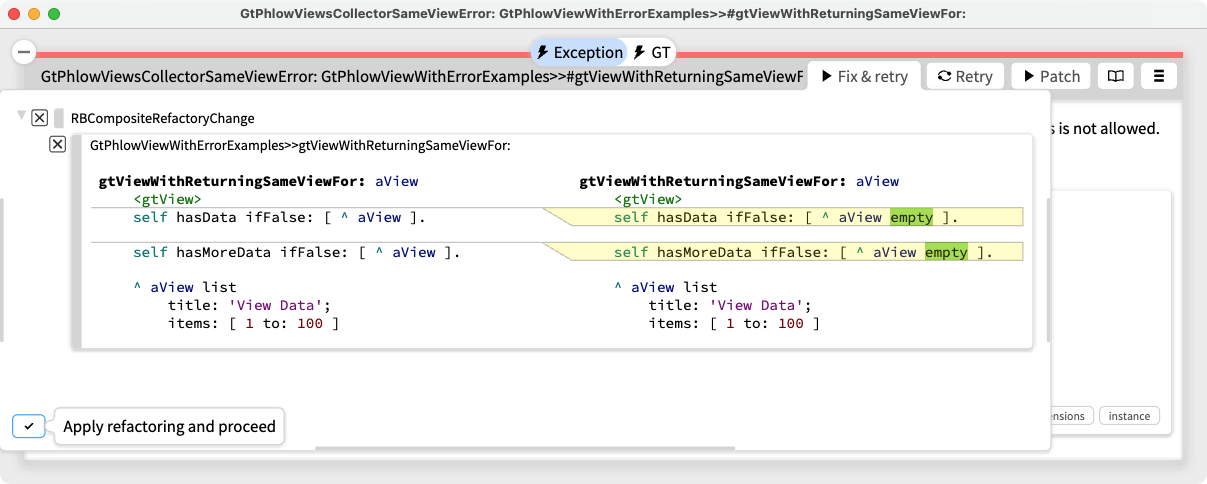
\includegraphics[width=\columnwidth]{emptyViewErrorFix}
  \caption{Transforming an empty view error.}
  \label{fig:emptyViewErrorFix}
\end{figure}
Clicking on the \emph{Apply refactoring and proceed} button will transform the source code, leave the debugger, and evaluate the rewritten code.
\steve{Fig. 14 and 15, it is not clear if the `aView` text that is highlighted is a modification of the picture that you did or a feature of GT (I think it is the latter). I would clarify it perhaps to not let the reader think that you try to show something without explaining what it is, but that it is just the (awesome) tool that does that. Or I'm wrong and you forgot to tell why you highlighted it ;)}

A custom debugger action, such as \emph{Fix it \& Proceed} or \emph{Retry} is defined in the same way as a custom debugger view: it is a method with a particular annotation, in this case being \st{<gtPhlowSameViewReturnDebugAction>} rather than \mbox{\st{<gtExceptionDebuggingView>}}, but  the mechanism is essentially the same.

The default behavior of such fixits is to open a debugger with the possibility of applying a proposed code transformation.
If, on the other hand, such code transformations should be applied automatically, this can be configured.
In our proof-of-concept implementation of moldable exceptions, this is done by evaluation the following code, which sets a flag in a globally accessible Singleton.
\begin{code}
GtMoldableExceptionTransformationsSettings defaultInstance allowAutomaticTransformations.
\end{code}
The \st{signal} method of exception classes can then optionally consult this flag to decide whether to spawn a debugger or apply the fix.
\ac{We can also generalize this a bit as the fix could not be just applying a transformation but also changing the state of the object at runtime. In this case we could also fix the error by replacing the returned view with a new instance of an empty view without changing the code. I'll add an example of such an action.}

As before, the custom debugger views and actions are mostly built from existing components, so the implementation effort is low.

\on{AC will check if we are allowed to describe here some of the LifeWare tests.}

% ============================================================
\section{Discussion and future directions}\label{sec:directions}

Moldable exceptions are just objects augmented with annotated methods that create alternative views and actions when they are used to spawn a moldable debugger.
The cost of creating these views and actions can be very low.
At the time of writing we have implemented some 26 custom debugger views, in an average of under 12 lines of code.
Over half of these are forwarding views that reuse (delegate to) existing views previously defined as object inspector views.
Several more are simple text, list or tree views, and only three create custom graphical widgets.

The simplest debugging views are just like inspector views, and many of our examples just forward (delegate) to existing views, but more generally exceptions have access to the reified run-time stack at the time that they are raised, so debugger views can extract and present arbitrary run-time information.
The \emph{Scripter steps} view we saw earlier in \autoref{fig:scripterStepsViewClicked} offers an example.
The same approach could be used, for example, to present or highlight just the ``interesting'' stack frames, for example in an event-driven application, just the methods that are responsible for processing events.
\on{AC: can you perhaps provide a better or more detailed example?}

At this time, moldable exceptions only offer the possibility to provide alternative views and actions, but not alternative ways to step through the execution.
\steve{Line 623, you say that "moldable exceptions only provide alternative views and actions but not alternative ways to step through the execution". I think you are partly wrong (sorry :P) but I think I heard someone saying or writing that GT was Pharo10-based. In Pharo10, if GT did not removed parts of the original system, you have Sindarin, which is exactly what we use it for. From our debugger extensions we use the API to script the stepping to write new stepping operators. In latest Pharo (11+12) we have for example an extended command that can skip part of code execution. So provided you write Sindarin scripts, you have this capability for free (does not mean it is simple, the smacc debugger stepping logic does not seem trivial to implement but I never tried). Perhaps what you meant there is that you do not have a "built-in" way in the moldable exceptions to build new stepping logics. But since it requires controlling the execution, at some point, you need to touch something low level (the interpreter) or use an API.}
Currently this is only possible by providing a completely separate debugger implementation.
In \autoref{fig:smaccDebugger} we see such a dedicated debugger for SmaCC~\cite{Brant17a}, the Smalltalk compiler compiler framework that has been spawned on an invalid fragment of Java code.
\begin{figure}[h]
  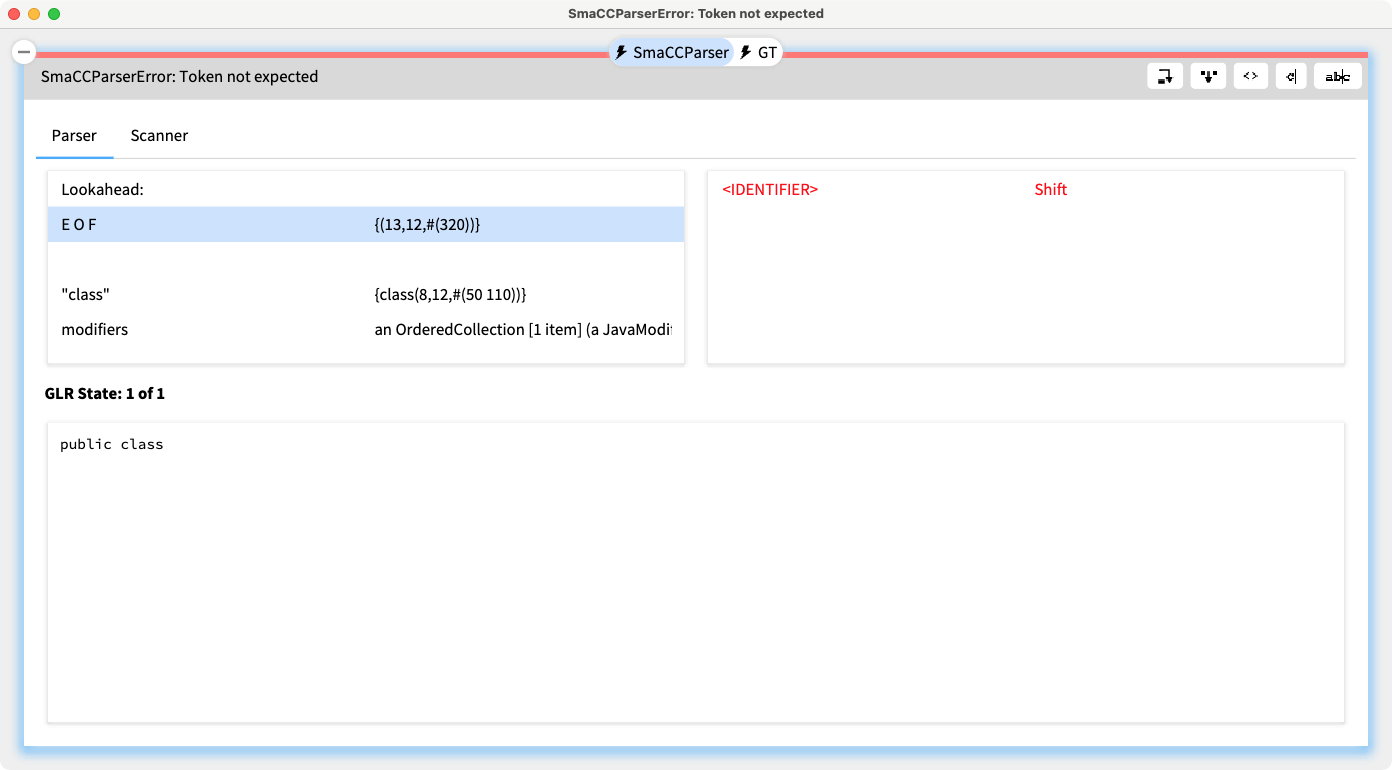
\includegraphics[width=\columnwidth]{smaccDebugger}
  \caption{A custom SmaCC debugger on an invalid Java snippet.}
  \label{fig:smaccDebugger}
\end{figure}
The SmaCC debugger offers the possibility to step through the grammar rules of a parser and explore its execution state.

\on{AC: is extending a debugger with custom stepping behavior something that we can foresee in the future? If so, what might it look like?}

Our proof-of-concept implementation of moldable exceptions presented here heavily leverages the existing infrastructure for moldable inspector views in \GT, but in principle there is nothing to prevent its application to other programming languages and IDEs.
The basic idea is simple: any moldable tool must be prepared, whenever it is created, to examine the execution context of the objects it is initialized with, and use that context to adapt its behavior.
In the case of a moldable debugger, this context is provided by the exception raised.
Custom debugger views and actions must then be provided by the specific exception raised.
One way to provide such views and actions is through specially annotated methods, but other means could be used, such as naming conventions, or a registry of debugger extensions.
The precise extension method will depend on the language technology available.
\on{More to say here?}

\on{Other future directions?}

\ac{As a side note.
Technically we have access to the raised exception just when initially opening the debugger.
Any step over action for example could lead to another exception being raises.
The standard behaviour in Pharo is to always open the debugger on an exception.
The default one is OupsNullException, but also in case an exception was explicitly raised doing a step into for example, changes the exception to the default one.
I think we should more or less also do that.
Currently we never change the exception that was raised in the debugger, even if when stepping we get another one.
Just we can extend that with the notion of the last “real” exception that was raised, and a history of exceptions raised in that debugging session.
Like that we could have step actions/view added by an exception that can be use as long as another explicit exception was not raised.}
\on{Can you write a paragraph explaining this?}

% ============================================================
\section{Related work}\label{sec:related}

\on{Are there other important references, and more recent ones, that we are missing?}

\steve{The Java Platform Debugger Architecture (JPDA) provides a 3-level architecture to build debuggers. The highest level is Java Debug Interface, basically you write a Java program that consumes VM stepping (and other) events. In the middle you have an interface to connect to the back end. Those two are to build new debuggers. With the lowest level, Java Virtual Machine Tools Interface (JVMTI), you can write agents that you attach to your debugger. In that sense, you can extend your debugger with new features. However with JVMTI you can only write in C or C++ (don't remember) so you have to write a debugger extension in another language than the one you debug and so you have to change worlds and manipulate very low-level concepts (cognitive cost) each time you observe something in your "home" language for which you want to extend your debugger. If you need a specific view, you need to build it from scratch and integrate it in your environment.}
\nocite{JVMTI24}

\steve{The VSCode debugger follows another philosophy, where you have a very standard debugger with very standard actions, but you can extend that debugger to support another back end for the language of your choice, so that your very specific language can benefit from super generic operations. For that it provides a protocol named Debugger Adapter Protocol (DAP).}
\nocite{DAP21}

\steve{The work of Bousse et al [1] follow the same path but for DSLs. They provide an environment to build DSLs execution engines, and for every DSL built with the environment, the environment provides a generic (time-traveling) debugger with the same features for all DSLs, except that the debugger will adapt to the stepping semantics of each DSLs. That semantic must be defined while designing and building the DSL, and is rather expansive to do (it is way harder than using introspection and intercession in Pharo like in the old GT-Debugger paper). They try to cope with that later by providing a "generic architecture" that allows them to build/extend specific debugging tools for DSLs [2] (they specifically speak about "Reducing the development cost of interactive debugger for DSLs"). They use the DAP to provide these new controls in VSCode. I don't think they provide views however. I'm not strong on this particular work though, it's worth re-reading it.}
% [1] Omniscient Debugging for Executable DSLs
% https://inria.hal.science/hal-01662336/file/jss17-debugging.pdf
\nocite{Bous18a}
% [2] Protocol-Based Interactive Debugging for Domain-Specific Languages
% https://hal.science/hal-04124727/document
\nocite{Enet23a}

\steve{In OUPS [3] a few years ago (that's an IWST paper, I like it but it's not top quality paper), we redesigned the way Pharo dealt with exceptions. It evolved since then and is better designed and more stable than at the time. We conditioned the opening of a debugger to the acceptance of both the debugger and the exception. In short, when an exception is raised the debugger system takes a list of available debuggers sorted by a priority property, and try to open the exception with each one of them until one debugger accepts the exception, and the exception accepts to be debugged by the debugger. We obtained two new capabilities:\\
- First at that time I was heavily working on the development of the current Pharo debugger, and it was unstable. When there was a bug in the debugger (which was often) I had no way to debug it. Fortunately, the GTDebugger was still there in the system. We created some kind of "meta-error", that was raised if an error originated from the opening of a debugger. That meta-error was debugged with the next-in-line debugger, so we could use another debugger to debug the failing debugger. For a long time that scenario was working so nice: I had a bug in the spec debugger, so it opened the GT-debugger that I used to debug the spec debugger and upon proceeding, the spec debugger opened working perfectly. GT was later removed.\\
- Second, we wanted to use it to open specific debuggers for specific exceptions. So you could have a domain exception that would accept only a specific debugger, or a specific debugger that would accept only specific exceptions. The problem is that we have to build complete debuggers for that (ie, at worst one debugger for each problem), which is why I guess we never applied this in real scenarios.}
% [3] Handling Error-Handling Errors: dealing with debugger bugs in Pharo
% https://inria.hal.science/hal-02992644/document 
\nocite{Cost20a}

\steve{A bit distant maybe, the work of Van de Vanter at al ([4]and [5]) where they extend the Truffle language implementation framework with "probes" that can extend the AST with introspection and (I think) intercession features. There are no views involved, but I remember the idea of extending the AST with new probes to easily build new debugging tools without touching low-level language concepts.}
% [4] Fast, Flexible, Polyglot Instrumentation Support for Debuggers and other Tools
% https://arxiv.org/ftp/arxiv/papers/1803/1803.10201.pdf
\nocite{Vant18a}
% [5] Building Debuggers and Other Tools: We Can “Have it All”
% https://vandevanter.net/mlvdv/publications/2015-icooolps.pdf
\nocite{Vant15a}

Early debuggers provided a command-line interface to inspect and step through the execution of a running program or a \emph{post mortem} ``core dump.''
With the advent of GUI-based IDEs, debuggers were also updated to offer interactive views to explore the execution state of a program and to step through its execution~\cite{Rose96a}.

% Debugging behavior
Studies of developer debugging behavior have shown that many developers have difficulty using debuggers and often shy away from them.
% Debugging: a review of the literature from an educational perspective
McCauley \etal report:
``We note, however, that our experiences with debugging tools is that many of them use execution traces as a method of assisting students to understand the execution of a program. Tubaishat~\cite{Tuba01a} characterized the use of execution traces as an example of a shallow reasoning technique''~\cite{McCa08a}.
% On the Dichotomy of Debugging Behavior Among Programmers
And Beller \etal note that
``Debuggers are difficult to use. Another reason given by interviewees, even though seasoned engineers, was that `the debugger is a complicated beast' (I2) and that `debuggers that are available now are certainly not friendly tools and they don't lend toward self-exploration'.''
\cite{Bell18a}

% Extensible debuggers
% A Simple and Extensible Graphical Debugger
An early example of an extensible debugger is \deet~\cite{Hans97a}.
Extensions to \deet were written Tcl/Tk or the Korn shell.
The focus of the extension mechanism in \deet is on adding new debugger features, rather than providing debugging support for specific application contexts.

% Extensible Debugger Framework for Extensible Languages
mbeddr~\cite{Voel17a} is a collection of languages and language extensions, mainly focusing on C, built with the Jetbrains MPS language workbench.
mbeddr includes an extensible debugger framework~\cite{Pavl15a} that focuses on providing support for the individual language extension, not application specific customizations.


% DSL Debugger extensions
There have been numerous efforts to develop specialized debuggers for domain-specific languages (DSLs) using a variety of approaches.
%  Grammar-Driven Generation of Domain-Specific Language Debuggers
Wu \etal report on grammar-driven generation of DSL debuggers~\cite{HuiW08a}.
% Declaratively Defining Domain-Specific Language Debuggers
Lindeman \etal leverage the Spoofax language workbench~\cite{Kats10a} to declaratively define DSL debuggers~\cite{Lind11a}.
% D2X: An eXtensible conteXtual Debugger for Modern DSLs
D2X~\cite{Brah23a} provides an API for DSLs to define debugger extensions.
All of these DSL debugger approaches focus on providing general debugging for a given DSL, not for more finely-grained application debugging issues.

% Sindarin: A versatile scripting API for the Pharo debugger
Sindarin is an extensible Pharo-based debugger that offers a rich API for scripting debugger extensions~\cite{Dupr19a}.
The use case for Sindarin is rather different from that of moldable exceptions, allowing developers to enter debugger scripts during a debugging session, rather than as a way to enable specialized debugger behavior in response to specific kinds of exceptions.

% Moldable tools
The Moldable Debugger~\cite{Chis15c} is an example of a \emph{moldable tool}~\cite{Chis17a} that adapts its behavior to a specific run-time application context.
The original moldable debugger, however, still required some significant implementation effort to define an alternative debugger interface, much like the other approaches we have cited from literature.
Similarly, the original moldable inspector~\cite{Chis15a} did not offer a very easy mechanism to provide custom inspector views depending on the object being inspected.
The adoption of the extension mechanism of using annotated methods to define inspector customizations led, over time, to the development of a large number of custom inspector views in the current version of \GT (over 3000 at last count).

% Historical
% Disciplined Exceptions
Disciplined use of exceptions is a well-established practice in object-oriented software development~\cite{Meye88a}.
The key insight and original contribution of moldable exceptions is to leverage exceptions as the hook to molding the behavior of the debugger.
No previous approach to extensible debuggers, including the original moldable debugger, has taken this approach.

%\ac{One argument reviewer B can bring :)), is that that exceptions are bad and should be avoided.
%We can also emphasize that when working with frameworks having dedicated exceptions can help developers understand what is happening.
%Users will not be exposed to exceptions, but developers need to reason about them.
%And if they can help, developers can actually have a bigger incentive to create custom exceptions.}\on{I think this is addressed now ...}

% ============================================================
\section{Conclusion}\label{sec:conclusion}

Debuggers are unloved beasts.
They provide a generic and clumsy interface to explore and debug the run-time state of a running program.
Many debugging problems can be better tackled by understanding the nature of the exception that was raised and caused the debugger to be activated.
Our key contribution is to show how a debugger can be dynamically molded with custom views and actions that depend on the specific exception raised.
The mechanism is lightweight, and many useful extensions can be defined with minimal implementation effort.

\on{What more can we say?}

%% The acknowledgments section is defined using the "acks" environment
%% (and NOT an unnumbered section).
%\begin{acks}
%To Robert, for the bagels and explaining CMYK and color spaces.
%\end{acks}

\bibliographystyle{ACM-Reference-Format}
\bibliography{moldableExceptions}


\end{document}
\endinput


\begin{inparaenum}[(i)]
	\item ...
\end{inparaenum}    
